% Internship Report -- FedGRAA
% Compile: tectonic --outdir build report.tex   (two passes handled internally)
% All personal/institutional specifics are <...> placeholders; see REPORTING_NOTES.md.
\documentclass[11pt,a4paper]{report}

\usepackage[margin=1in]{geometry}
\usepackage[T1]{fontenc}
\usepackage[utf8]{inputenc}
\usepackage{graphicx}
\usepackage{booktabs}
\usepackage{array}
\usepackage{amsmath,amssymb,amsthm}
\usepackage{algorithm}
\usepackage{algpseudocode}
\usepackage{caption}
\usepackage{subcaption}
\usepackage{cite}
\usepackage{enumitem}
\usepackage{titlesec}
\usepackage{setspace}
\usepackage{microtype}
\usepackage{xurl}
\usepackage{fancyhdr}
\usepackage[colorlinks=true,linkcolor=black,citecolor=black,urlcolor=blue,bookmarksnumbered]{hyperref}

% ---------- layout ----------
\setstretch{0.95}
\setlength{\parskip}{1.5pt plus 0.5pt}
\setlength{\parindent}{1.5em}
\captionsetup{font=small,labelfont=bf,skip=4pt}
\setlist{nosep,leftmargin=1.5em}
% tighten float spacing for the page budget
\setlength{\textfloatsep}{7pt plus 1pt minus 2pt}
\setlength{\intextsep}{6pt plus 1pt minus 2pt}
\setlength{\floatsep}{6pt plus 1pt minus 2pt}
\setlength{\abovecaptionskip}{3pt}
\renewcommand{\arraystretch}{0.92}

% chapters start closer to the top; consistent with a 20-25 page target
\titleformat{\chapter}[display]
  {\normalfont\huge\bfseries}{\chaptertitlename\ \thechapter}{16pt}{\huge}
\titlespacing*{\chapter}{0pt}{-14pt}{18pt}
\titlespacing*{\section}{0pt}{10pt}{6pt}
\titlespacing*{\subsection}{0pt}{8pt}{5pt}
\titlespacing*{\subsubsection}{0pt}{7pt}{4pt}

\pagestyle{fancy}
\fancyhf{}
\fancyhead[L]{\small\nouppercase{\leftmark}}
\fancyhead[R]{\small\thepage}
\renewcommand{\headrulewidth}{0.4pt}
\fancypagestyle{plain}{\fancyhf{}\fancyfoot[C]{\small\thepage}\renewcommand{\headrulewidth}{0pt}}

\newtheorem{theorem}{Theorem}[chapter]
\newtheorem{proposition}{Proposition}[chapter]

% ---------- placeholder marker: renders as <Text> in angle brackets ----------
\newcommand{\ph}[1]{$\langle$\textit{#1}$\rangle$}

% ---------- notation ----------
\newcommand{\simplex}{\Delta}
\newcommand{\proj}{\Pi_{\simplex}}
\newcommand{\Lprime}{L'}

\begin{document}

% =====================================================================
%  FRONT MATTER (roman folios)
% =====================================================================
\pagenumbering{Alph}

% ---------------- Title page ----------------
\begin{titlepage}
\centering
{\large \textsc{Internship Report}}\\[1.6em]
{\LARGE\bfseries Federated Gradient-Refined Adaptive Averaging for Intrusion Detection:\\[0.35em]
Faithful Reproduction, Convergence Defect Diagnosis, and a Privacy-Compliant Extension (FedGRAA-v2)\par}
\vspace{1.8em}
{\large \textit{A report submitted in partial fulfilment of the requirements\\ for the research internship}}\\[2.2em]
{\large \textit{submitted by}}\\[0.5em]
{\large \textbf{Nikhil Pravin Pise}}\\
{Roll No.: \ph{Roll No.}}\\
{\ph{Department}, \ph{Home Institution}}\\[2.2em]
{\large \textit{under the guidance of}}\\[0.5em]
{\textbf{\ph{Professor Name}}}\\
{\ph{Department}, Indian Institute of Technology Guwahati}\\[0.8em]
{\large \textit{and day-to-day mentorship of}}\\[0.5em]
{\textbf{\ph{Mentor Name}}}\\[2.2em]
{\ph{Department}}\\
{\ph{Home Institution}}\\[0.8em]
{\ph{Place} \textbullet\ \ph{Month Year}}
\end{titlepage}
\pagenumbering{roman}

% ---------------- Certificate ----------------
\chapter*{Certificate}
\phantomsection\addcontentsline{toc}{chapter}{Certificate}
\thispagestyle{plain}

{\sloppy
This is to certify that the work contained in this internship report entitled
\textbf{``Federated Gradient-Refined Adaptive Averaging for Intrusion
Detection: Faithful Reproduction, Convergence Defect Diagnosis, and a
Privacy-Compliant Extension (FedGRAA-v2)''}, submitted by \textbf{Nikhil
Pravin Pise} (Roll No.: \ph{Roll No.}), \ph{Department}, \ph{Home
Institution}, is a bonafide record of the research internship carried out by
him under the supervision of \ph{Professor Name}, \ph{Department}, Indian
Institute of Technology Guwahati, and the day-to-day mentorship of
\ph{Mentor Name}, during the period \ph{Start Date} to \ph{End Date}.
\par}

\vspace{4em}
\noindent\begin{tabular}{@{}p{0.45\textwidth}p{0.45\textwidth}@{}}
\rule{0.8\linewidth}{0.4pt} & \rule{0.8\linewidth}{0.4pt}\\[0.3em]
\ph{Mentor Name} & \ph{Professor Name}\\
Day-to-day Mentor & Professor\\
& \ph{Department}, IIT Guwahati\\[1.5em]
Date: \ph{Date} & Date: \ph{Date}\\
Place: \ph{Place} & Place: \ph{Place}\\
\end{tabular}

% ---------------- Acknowledgement ----------------
\chapter*{Acknowledgement}
\phantomsection\addcontentsline{toc}{chapter}{Acknowledgement}
\thispagestyle{plain}

I thank \ph{Professor Name}, \ph{Department}, Indian Institute of Technology
Guwahati, for accepting me as a research intern and for the direction that
shaped this work, and \ph{Mentor Name} for day-to-day mentorship throughout the
internship, including the reproduce-then-audit discipline that defines the
results reported here. I thank \ph{Home Institution} for supporting this
internship period.

Parts of the literature triage, drafting, and code development in this
internship used AI-assistant tooling under my direction; every reported number
was produced by, and independently re-verified against, the compute artifacts
in the accompanying repository.

\begin{flushright}
\textbf{Nikhil Pravin Pise}\\
\ph{Place}, \ph{Month Year}
\end{flushright}

% ---------------- Abstract ----------------
\chapter*{Abstract}
\phantomsection\addcontentsline{toc}{chapter}{Abstract}
\thispagestyle{plain}

% PLACEHOLDER-ABSTRACT (numbers verified against results/ artifacts)
\noindent
This report documents a research internship on federated-learning intrusion
detection: faithfully reproduce the FedGRAA adaptive-aggregation method,
explain any divergence from its reported results, correct its convergence
theory, and design a privacy-compliant extension. Reproducing the printed
algorithm exactly, I measured 0.00\% rare-class accuracy on CIC-IDS-2017
against the manuscript's claimed 88.88\% (33.33\% reproduced on UNSW-NB15
against 21.09\% claimed). A mechanistic diagnosis traced the divergence to a
missing simplex-projection step: the learned aggregation weight leaves the
probability simplex in round 1 in all 120 unprojected cells, turning the
aggregation into unbounded affine extrapolation and violating the paper's own
convergence lemma. A minimal two-part correction recovers 89.3\%/69.2\%
rare-class accuracy, and the guarantee was restated as gradient-mapping
stationarity $O(1/T)+O(\zeta^2)$ under a Polyak-{\L}ojasiewicz condition. The
extension, FedGRAA-v2, removes the design's two privacy violations through a
secure-aggregation protocol reconstructing the exact composite-loss gradient,
reaching 93.47\%/69.66\% rare-class accuracy across 960 cells at
6.00$\times$-to-3.00$\times$ communication cost, with 111/112 paired
significance tests rejecting the null. An adversarial evaluation shows the
same up-weighting mechanism is exploitable and that successfully defended
cells collapse rare-class recall to near 0\% - a trade-off none of the
evaluated defenses avoids.

% ---------------- TOC / LoF / LoT ----------------
{\hypersetup{linkcolor=black}
\tableofcontents
\clearpage
\phantomsection\addcontentsline{toc}{chapter}{List of Figures}
\listoffigures
\vspace{1.5em}
{\let\clearpage\relax\let\cleardoublepage\relax
\phantomsection\addcontentsline{toc}{chapter}{List of Tables}
\listoftables}
}

% ---------------- Nomenclature ----------------
\chapter*{Nomenclature}
\phantomsection\addcontentsline{toc}{chapter}{Nomenclature}
\thispagestyle{plain}

\noindent\textbf{Roman capitals}
\begin{center}
\begin{tabular}{@{}p{0.18\textwidth}p{0.76\textwidth}@{}}
$B$ & client mini-batch size (64)\\
$D_k$, $|D_k|$ & client $k$'s local dataset and its size\\
$D_V$; $D_V^{h,m,n}$ & held-out validation data; pooled set and head/median/rare-class strata\\
$E$, $E'$ & local training epochs (2); weight-refinement inner epochs (5)\\
$G_{\eta'}(w)$ & projected gradient mapping at step size $\eta'$\\
$K$ & number of participating clients (14 CIC-IDS-2017; 9 UNSW-NB15)\\
$L_k$ & client $k$'s local loss\\
$L_h$, $L_m$, $L_u$ & validation losses on the head, median, and rare-class strata\\
$L_a$ & common-class loss, the lower of the two common strata, $\min(L_h,L_m)$\\
$\Lprime$ & composite objective $(1-\gamma)L_a+\gamma L_u$\\
$P$, $P_k$ & flattened model parameters; client $k$'s contribution\\
$S_t$ & client set selected at round $t$\\
$T$ & total communication rounds (200)\\
\end{tabular}
\end{center}

\noindent\textbf{Roman lowercase}
\begin{center}
\begin{tabular}{@{}p{0.18\textwidth}p{0.76\textwidth}@{}}
$c_k$ & client $k$'s count-weighted contribution to the composite gradient\\
$d$ & Cohen's effect size (paired Wilcoxon comparisons); model input width\\
$f$ & tolerable client dropout/collusion fraction ($f < K/3$)\\
$m$ & gradient-refresh interval for the federated backward pass\\
$n$ & number of protected rare classes (3)\\
$n_{\mathrm{arm}}$, $n_n$ & SecAgg-pooled counts of the common and rare strata\\
$n_{\mathrm{arm},k}$, $n_{n,k}$ & client $k$'s own counts in those strata\\
$t$ & SecAgg reconstruction threshold (default $\lfloor K/2\rfloor+1$)\\
$w$, $w_k$ & learned aggregation-weight vector; client $k$'s weight\\
\end{tabular}
\end{center}

\noindent\textbf{Greek letters}
\begin{center}
\begin{tabular}{@{}p{0.18\textwidth}p{0.76\textwidth}@{}}
$\beta_{\mathrm{eff}}$ & effective smoothness constant of the composite objective\\
$\gamma$ & personalization coefficient trading common-class vs rare-class loss\\
$\simplex$ & probability simplex $\{w\in\mathbb{R}^K:w_k\ge0,\sum_k w_k=1\}$\\
$\varepsilon$, $\delta$ & differential-privacy budget parameters\\
$\zeta$, $\tilde{\zeta}$ & inexactness bound of the gradient oracle; its measured value\\
$\eta$, $\eta'$ & client learning rate (0.01); weight learning rate (0.1 literal, 0.01 corrected)\\
$\eta_{\mathrm{fake}}$ & attacker fake-update step size in the signature attack\\
$\theta_g$, $\theta_k$ & global model parameters; client $k$'s local parameters\\
$\theta'_g$ & candidate aggregate broadcast for the federated backward pass\\
$\proj$ & Euclidean projection onto $\simplex$ (Duchi et al.)\\
$\sigma$ & per-seed standard deviation of an adversarial metric\\
\end{tabular}
\end{center}

\noindent\textbf{Acronyms}
\begin{center}
\begin{tabular}{@{}p{0.18\textwidth}p{0.76\textwidth}@{}}
ASR & attack success rate\\
CI & confidence interval\\
DP & differential privacy\\
FedGRAA & Federated Gradient-Refined Adaptive Averaging\\
FL & federated learning\\
IDS, NIDS & (network) intrusion detection system\\
IID, non-IID & (non-)independent and identically distributed\\
MLP & multilayer perceptron\\
PL & Polyak-{\L}ojasiewicz (condition)\\
SecAgg & secure aggregation\\
\end{tabular}
\end{center}

\clearpage
\pagenumbering{arabic}

% =====================================================================
%  CHAPTER 1 -- INTRODUCTION
% =====================================================================
\chapter{Introduction}
\label{ch:intro}

\section{Motivation}
\label{sec:motivation}

An intrusion detection system (IDS) monitors network traffic to detect and
help prevent attacks. Traditional IDS deployments depend on \emph{centralized}
data collection: traffic from every monitored network is pooled at one site
and a detection model is trained on the aggregate. That centralization is the
deployment blocker. Raw network telemetry is among the most privacy-sensitive
data an organization holds; pooling it across organizational boundaries is
frequently prohibited, and it concentrates breach risk at a single point.
Federated learning (FL) removes the pooling requirement entirely: each
participating site trains a local model on its own traffic and shares only
model parameters with a coordinating server, which aggregates them into a
global model \cite{mcmahan2017fedavg,kairouz2021fl}.

FL's own aggregation rule, however, creates a second problem specific to
intrusion detection. The standard aggregator, FedAvg, weights each client's
contribution by its local dataset size alone, under the assumption that client
data is roughly homogeneous and balanced. Real network telemetry is not: some
clients see frequent, common intrusions such as port scans and denial of
service, while the attack classes that matter most operationally -
infiltration, SQL injection, Heartbleed-class exploits - are exactly the ones
seen rarely, by few clients, in small quantity. Under size-proportional
weighting, a client holding the only handful of examples of a rare attack
class has negligible influence on the aggregate, however informative its
gradient is for that class. The global model's ability to detect the rarest,
highest-consequence attacks degrades accordingly. This is a structural
under-representation problem, not a training-instability problem.

FedGRAA \cite{fedgraa-paper} targets this directly: it replaces the fixed
size-proportional weight with a learned, $\gamma$-tunable aggregation weight
that is re-optimized every round against a composite validation objective
explicitly separating common-class and rare-class loss.

\section{The internship project}
\label{sec:project}

The internship reproduced the published FedGRAA method - \emph{``Federated
Gradient-Refined Adaptive Averaging for Intrusion Detection Systems''}
\cite{fedgraa-paper}, a manuscript under review at the time of writing - from
scratch in TensorFlow/Keras, measured its claims honestly, diagnosed the
divergences found, corrected its convergence theory, and designed a novel
privacy-compliant extension. The work proceeded in three stages:

\begin{description}
\item[Stage A - faithful reproduction.] Re-implement the printed algorithm
exactly, including its stated datasets, architecture, and hyperparameters,
with every experiment cell persisted to a provenance-embedded artifact.
\item[Stage B - critique, corrected theory, and ablation.] Root-cause the
reproduction's divergences mechanistically, restate the convergence guarantee
correctly, and isolate which design element is responsible for which failure
via a controlled ablation.
\item[Stage C - extension.] Remove the design's two structural privacy
violations in a privacy-compliant redesign (FedGRAA-v2), and evaluate it
against the full baseline frontier including adversarial robustness.
\end{description}

The internship was carried out under the supervision of an IIT Guwahati
professor with day-to-day PhD-student mentorship. All implementation and
experimental artifacts are in the accompanying repository.

\section{Objectives}
\label{sec:objectives}

The work was scoped to five objectives, each of which maps to a results
section of Chapter~\ref{ch:results}:

\begin{enumerate}[label=\textbf{O\arabic*.}]
\item \textbf{Faithful reproduction with persisted artifacts} - re-implement
the published algorithm exactly and reproduce its reported headline results,
or measure the gap precisely (Section~\ref{sec:stagea}).
\item \textbf{Root-cause any divergence mechanistically} - not merely observe
that reproduction differs from claim, but identify the design element
responsible and demonstrate it causally (Section~\ref{sec:diagnosis}).
\item \textbf{Correct the convergence theory} - restate the guarantee the
actual (non-convex, constrained) system supports, and validate the minimal
algorithmic fix with statistical rigor across seeds (Section~\ref{sec:stageb}).
\item \textbf{Remove the design's privacy violations} - the mechanism as
published requires the server to already know which classes are rare and to
hold a pooled labelled validation set, both in tension with FL's
decentralization premise; the extension must eliminate both without changing
the objective (Sections~\ref{sec:v2methodology} and \ref{sec:stagec}).
\item \textbf{Evaluate against the full baseline frontier, including
adversarial robustness} - 19 methods over 10 seeds with paired significance
testing, plus a measured attack-surface analysis of the mechanism itself
(Sections~\ref{sec:stagec}--\ref{sec:adversarial}).
\end{enumerate}

\section{Summary of contributions}
\label{sec:contributions}

\begin{enumerate}
\item \textbf{The defect.} A mechanistic diagnosis showing the printed
FedGRAA weight update has no mechanism to remain a valid convex combination:
the learned weight leaves the probability simplex in round 1 in all 120
unprojected experiment cells, turning aggregation into unbounded affine
extrapolation and invalidating the paper's own convergence lemma
(Sections~\ref{sec:fedgraa-defect}, \ref{sec:diagnosis}).
\item \textbf{The fix.} A minimal correction - Euclidean projection onto the
simplex plus a tenfold-smaller weight learning rate - that restores
rare-class accuracy to 89.3\%/69.2\% on the two benchmarks, validated across
10 seeds in a $2\times2$ factorial ablation (Section~\ref{sec:stageb}).
\item \textbf{The corrected theorem.} A restated convergence guarantee:
gradient-mapping stationarity $O(1/T)+O(\zeta^2)$ under a
Polyak-{\L}ojasiewicz condition, extended to the inexact gradient oracle of
the privacy-compliant design (Section~\ref{sec:corrected-theory}).
\item \textbf{FedGRAA-v2.} A privacy-compliant redesign that replaces both
oracle assumptions - server knowledge of which classes are rare, and a
server-held labelled validation set - with a secure-aggregation two-phase
protocol reconstructing the \emph{exact} composite-loss gradient
(Section~\ref{sec:v2methodology}).
\item \textbf{The evaluation, including honest negative results.} A 960-cell
campaign (10 seeds on the 830-cell main grid, 5 on the T7/T7G arms) against
19 baselines (93.47\%/69.66\% best rare-class accuracy; 111 of 112 paired
significance tests rejecting the null) plus an
adversarial evaluation finding that the up-weighting mechanism is exploitable
by construction and that defended cells collapse rare-class recall to near
0\% - a trade-off no evaluated defense avoids (Sections~\ref{sec:stagec},
\ref{sec:adversarial}).
\end{enumerate}

\section{Outline of the report}
\label{sec:outline}

Chapter~\ref{ch:related} reviews federated learning, adaptive aggregation,
robust aggregation, and poisoning attacks and defenses in federated intrusion
detection, and positions the present work. Chapter~\ref{ch:methodology}
presents the problem formulation, FedGRAA as published, the diagnosed defect,
the minimal correction, the corrected convergence theory, and the FedGRAA-v2
extension. Chapter~\ref{ch:results} reports the staged experimental results:
reproduction, diagnosis, ablation, the FedGRAA-v2 frontier, significance,
overhead, and adversarial robustness. Chapter~\ref{ch:discussion} discusses
implications and limitations. Chapter~\ref{ch:conclusion} concludes and
outlines future work.

% =====================================================================
%  CHAPTER 2 -- RELATED WORK
% =====================================================================
\chapter{Related Work}
\label{ch:related}

\section{Federated learning and FedAvg}
\label{sec:fedavg}

FL trains a global model across decentralized clients without sharing local
data. At round $t$, the server broadcasts $\theta_g^t$ to a fixed client set
$S_t$; client $k$ starts from the broadcast $\theta_g^t$ and runs local
optimization for $E$ epochs on its own data $D_k$,
\begin{equation}
\theta_k^{(e+1)} \leftarrow \theta_k^{(e)} - \eta\, \nabla L_k(\theta_k^{(e)}; b),
\quad \theta_k^{(0)} = \theta_g^t,\ \ e = 0,\dots,E{-}1,
\label{eq:local-sgd}
\end{equation}
returning $\theta_k^{t+1} = \theta_k^{(E)}$; and the server aggregates by
dataset-size-proportional weighting,
FedAvg \cite{mcmahan2017fedavg}:
\begin{equation}
\theta_g^{t+1} = \sum_{k \in S_t} \frac{|D_k|}{|D|}\, \theta_k^{t+1}
\label{eq:fedavg}
\end{equation}

\begin{algorithm}[htbp]
\caption{Federated round (FedAvg; the loop FedGRAA modifies)}
\label{alg:fedavg}
\begin{algorithmic}[1]
\For{$t = 1 \dots T$}
  \State server broadcasts $\theta_g^t$ to clients $k \in S_t$
  \State each client runs $E$ local epochs (Eq.~\eqref{eq:local-sgd}),
    returns $\theta_k^{t+1}$
  \State server aggregates $\theta_g^{t+1} \gets \sum_k (|D_k|/|D|)\,
    \theta_k^{t+1}$ (Eq.~\eqref{eq:fedavg})
\EndFor
\end{algorithmic}
\end{algorithm}

The global objective is the size-weighted average of local losses,
$L(\theta)=\sum_k (|D_k|/|D|)L_k(\theta)$. Under Eq.~\eqref{eq:fedavg} a
client's influence on $\theta_g$ is \emph{exactly} proportional to $|D_k|$.
Under non-IID data - in particular when the classes that matter most are held
by the smallest-data clients - this systematically dilutes their contribution.

\section{Adaptive aggregation}
\label{sec:adaptive-agg}

Adaptive aggregation weighting has converged on three signal families:
alignment with the global update direction (FedAWA \cite{fedawa}), client
loss or accuracy (FedNolowe \cite{fednolowe}, PACT \cite{pact}), and
statistical outlier filtering (MESAS \cite{mesas}, CrowdGuard
\cite{crowdguard}, FreqFed \cite{freqfed}). Related adaptive rules in the
same space include FedAPA \cite{fedapa}, DA-PFL \cite{dapfl}, FedMADE
\cite{fedmade} and XAI-SOH-FL \cite{xaisohfl}. In imbalanced intrusion
detection, all three systematically suppress exactly the clients FedGRAA is
designed to protect: divergent, high-loss, minority-class clients holding
the rarest attacks look identical, under these signals, to noise or
attackers.

\section{The counter-current}
\label{sec:counter-current}

A counter-current to suppressing unusual updates exists. FedAWARE
\cite{fedaware} maximizes gradient \emph{diversity} rather than penalizing
it. Jiang et al.\ \cite{jiang2024} and AdaAggRL \cite{adaaggrl} learn weights
via reinforcement learning that explicitly protect rare contributions from
being filtered out. CELM \cite{celm} up-weights clients with discriminative
evidence for underrepresented classes via data-free logit-maximization
probing, requiring no server-held validation data; SpectralFed
\cite{spectralfed} and CoAst \cite{coast} estimate contribution data-free via
gradient spectral entropy and update-sign agreement. Precision-weighted
aggregation \cite{reyes2021} derives weights from gradient variance. In
intrusion detection specifically, FedPGO \cite{fedpgo} reweights clients by
gradient orthogonality on CIC-IDS-2017 - the same domain, the same dataset, a
closely related mechanism family - and NIDS-FGPA \cite{nidsfgpa} weights by
gradient similarity for communication efficiency.

\section{Trust-based robust aggregation}
\label{sec:trust-based}

FLTrust \cite{fltrust}, RAGA \cite{raga}, and FedTruth \cite{fedtruth} all
assume, in one form or another, a server-held reference - a root dataset
(FLTrust) or a trusted validation anchor - structurally identical to the
$D_V$ dependency the original FedGRAA shares and FedGRAA-v2 removes. FedTruth
explicitly calls this assumption impractical; CoAst independently describes a
server reference set as ``difficult to obtain in practical FL scenarios;''
CELM's own abstract restates the concern. This is a known, common, fixable
shortcut across the adaptive-aggregation literature, not a defect specific to
FedGRAA.

\section{Classic optimizers and poisoning defenses}
\label{sec:poisoning}

FedAvg \cite{mcmahan2017fedavg}, FedProx \cite{fedprox}, FedOpt
\cite{reddi2021fedopt}, SCAFFOLD \cite{scaffold} and FedNova \cite{fednova}
are the field-standard, non-personalization-aware optimizers: they correct
systems and statistical heterogeneity in the generic sense, but none carries
an explicit rare-class objective, and they are evaluated here as context
rather than as the primary competitor set.

FL's openness creates a poisoning surface: malicious clients can submit
label-flipped or directly model-poisoned updates (the ``pill'' attack of Guo
et al.\ \cite{guo2026pill}). Published defenses in the NIDS domain include
SecFedNIDS \cite{secfednids}, a consensus-filter/SOS defense evaluated on
UNSW-NB15, SB-FedNIDS \cite{sbfednids}, which targets class imbalance
directly, and WeiDetect \cite{weidetect}, evaluated against a comparable
threat model; Ma et al.\ \cite{mayang2026} survey the wider
aggregation-defense landscape. None of these - nor any adjacent adaptive-aggregation method
above - asks the question this internship's adversarial evaluation asks
directly: does an aggregation rule that deliberately up-weights statistically
unusual client contributions thereby create an attack surface an adversary
can exploit by construction? AdaAggRL \cite{adaaggrl}, whose RL-learned
weighting is explicitly framed as adversarially robust, is the closest
adjacent design and is reused unmodified as a third defense arm.

\section{Positioning}
\label{sec:positioning}

FedGRAA sits inside the counter-current of Section~\ref{sec:counter-current},
at a point none of these methods occupies: a single-global-model aggregation
rule with an explicit $\gamma$-tunable trade-off between rare-class emphasis
and conventional size-proportional weighting, an exact (not approximated)
gradient against the rare-class objective, and evaluation on rare-class
recall specifically - the axis the related methods' own papers do not report.
The claim is not that this region is unoccupied - FedPGO occupies an adjacent
point on the same dataset - but that this specific point is unreported, and
Chapter~\ref{ch:results} evaluates it against the closest fourteen
competitors plus five classic optimizers directly, rather than asserting the
gap.

% =====================================================================
%  CHAPTER 3 -- PROPOSED METHODOLOGY
% =====================================================================
\chapter{Proposed Methodology}
\label{ch:methodology}

This chapter carries the internship's technical core: what the printed
algorithm specifies (Section~\ref{sec:problem}, \ref{sec:fedgraa-printed}),
the defect found in it (Section~\ref{sec:fedgraa-defect}), the minimal
correction (Section~\ref{sec:correction}), the corrected convergence theory
(Section~\ref{sec:corrected-theory}), the FedGRAA-v2 privacy-compliant
redesign (Section~\ref{sec:v2methodology}), the attack surface the mechanism
itself creates (Section~\ref{sec:attack-surface}), and the verification
discipline the results rest on (Section~\ref{sec:verification}).

\section{Problem formulation}
\label{sec:problem}

An FL system trains a global model over $K$ clients that never share raw
data. Each round $t$, the server broadcasts $\theta_g^t$; client $k$ updates
locally (Eq.~\eqref{eq:local-sgd}) and returns $\theta_k^{t+1}$; the server
aggregates. FedGRAA replaces Eq.~\eqref{eq:fedavg}'s fixed size-proportional
weighting with a learned weight vector $w^t$ constrained - in intent - to the
probability simplex
\begin{equation}
\simplex = \bigl\{ w \in \mathbb{R}^K : w_k \ge 0,\ \textstyle\sum_k w_k = 1 \bigr\},
\label{eq:simplex}
\end{equation}
so that $\theta_g^{t+1}=\sum_k w_k^t\,\theta_k^{t+1}$ is a convex combination.

Each round, the server forms a candidate aggregate
$\theta'_g=\sum_k w_k^{t-1}\theta_k^t$ using the previous round's weights,
then refines $w$ for $E'$ inner epochs against a composite validation loss
that explicitly separates common-class and rare-class performance:
\begin{align}
L_a &= \min\bigl(L_h(\theta'_g; D_V^h),\, L_m(\theta'_g; D_V^m)\bigr)
\label{eq:la}\\
\Lprime(\theta'_g) &= (1-\gamma)\, L_a(\theta'_g; D_V^h, D_V^m)
                   + \gamma\, L_u(\theta'_g; D_V^n)
\label{eq:lprime}
\end{align}
where $D_V^h$/$D_V^m$ are validation data split at the median class frequency
and $D_V^n$ is held-out data for the $n$ rarest classes. The personalization
coefficient $\gamma\in[0,1]$ sets the trade-off: $\gamma\to1$ prioritizes the
rare-class loss $L_u$; $\gamma\to0$ recovers ordinary size-agnostic
behaviour. The $n$ rarest classes are, in the published design, an oracle
list the server is assumed to know in advance. The weight gradient follows
the chain rule through the aggregate: since
$\theta'_g=\sum_k w_k P_k$ with $P_k$ the flattened client parameters,
\begin{equation}
\frac{\partial \Lprime}{\partial w_k}
= \bigl\langle \nabla_P \Lprime(\theta'_g),\, P_k \bigr\rangle .
\label{eq:wgrad}
\end{equation}

\section{FedGRAA as published}
\label{sec:fedgraa-printed}

Algorithm~\ref{alg:fedgraa-printed} states the weight update \emph{as
printed} in the reproduced manuscript, including the Adam optimizer the
manuscript's own experimental section specifies for both the client update
and the weight update (confirmed by its correction note and by the reference
implementation, which labels this line ``Adam step on $w$ (eq.~10)'').

\begin{algorithm}[htbp]
\caption{FedGRAA weight update - as printed (defective)}
\label{alg:fedgraa-printed}
\begin{algorithmic}[1]
\Procedure{FedGRAA}{$\theta_k^t,\, w^{t-1}$}
  \For{$e = 1 \dots E'$}
    \State $\theta'_g \gets \sum_k w_k^{t-1,e}\, \theta_k^t$
    \State $L_a \gets \min\bigl(L_h(\theta'_g; D_V^h),\, L_m(\theta'_g; D_V^m)\bigr)$
    \State $\Lprime \gets (1-\gamma)\, L_a + \gamma\, L_u(\theta'_g; D_V^n)$
    \State $g \gets \nabla_w \Lprime(\theta'_g)$ \Comment{Eq.~\eqref{eq:wgrad}}
    \State $w^{t-1,e} \gets \Call{Adam-step}{w^{t-1,e-1},\, g}$
  \EndFor
  \State \Return $w^t \gets w^{t-1,E'}$ \Comment{no projection - see Section~\ref{sec:fedgraa-defect}}
\EndProcedure
\end{algorithmic}
\end{algorithm}

The initial weights use static reparameterization - inverse-size weighting
$w_k^0\propto 1/|D_k|$ - a fixed control that over-corrects toward small
clients without adaptivity:
\begin{equation}
\theta_g^{t+1} = \sum_k \left[\frac{1/|D_k|}{\sum_j 1/|D_j|}\right] \theta_k^{t+1}
\label{eq:static-reparam}
\end{equation}

\section{The diagnosed defect}
\label{sec:fedgraa-defect}

The headline internship finding is that Algorithm~\ref{alg:fedgraa-printed}
has \textbf{no mechanism to remain a valid convex combination}. The Adam
update on $w$ is unconstrained: nothing projects $w$ back onto $\simplex$
after the inner-epoch refinement. Section~\ref{sec:diagnosis} shows
empirically that this is not a cosmetic gap - $w$ leaves the simplex in round
1 in all 120 unprojected experiment cells, at every $\gamma$, on both
datasets, with zero exceptions. Once $w\notin\simplex$, the ``weighted
average'' $\sum_k w_k\theta_k$ is no longer a convex combination but an
unbounded affine extrapolation, and the composite loss it produces can - and
does - diverge.

The manuscript's own Appendix~A.1 convergence proof cannot cover this
behaviour, for three independent reasons:
\begin{enumerate}
\item its convexity assumption on $\Lprime$ is false for the paper's own
stated tanh-MLP loss surface;
\item the composite term $L_a=\min(L_h,L_m)$ is non-smooth exactly in the
region training drives the iterate toward; and
\item its Lemma~2 tacitly assumes $w\in\simplex$ - the very property the
printed update does not maintain - so the proof's premise is violated from
round 1.
\end{enumerate}

\section{The minimal correction}
\label{sec:correction}

The minimal change that restores the intended behaviour is an explicit
Euclidean projection onto the simplex after the inner-epoch refinement, plus
a tenfold-smaller weight learning rate $\eta'=0.01$ (the literal 0.1
overshoots the simplex boundary in a single step). With Duchi et al.'s
\cite{duchi2008projection} projection:
\begin{equation}
w^t = \proj\bigl(w^{t-1,E'} - \eta'\, \partial \Lprime(w^{t-1,E'})\bigr),
\label{eq:projected-update}
\end{equation}
implemented as Algorithm~\ref{alg:fedgraa-corrected}; $E'=5$ is unchanged.
This corrected variant was kept strictly diagnostic - it is evaluated against
the literal arm in Section~\ref{sec:stageb} but never merged into the
reproduction baseline, so the reproduction numbers of
Section~\ref{sec:stagea} remain a faithful measurement of the printed
algorithm.

\begin{algorithm}[htbp]
\caption{FedGRAA weight update - corrected (proposed)}
\label{alg:fedgraa-corrected}
\begin{algorithmic}[1]
\Procedure{FedGRAA}{$\theta_k^t,\, w^{t-1}$}
  \For{$e = 1 \dots E'$}
    \State $\theta'_g \gets \sum_k w_k^{t-1,e}\, \theta_k^t$
    \State $L_a \gets \min\bigl(L_h(\theta'_g; D_V^h),\, L_m(\theta'_g; D_V^m)\bigr)$
    \State $\Lprime \gets (1-\gamma)\, L_a + \gamma\, L_u(\theta'_g; D_V^n)$
    \State $g \gets \nabla_w \Lprime(\theta'_g)$
    \State $w^{t-1,e} \gets \Call{Adam-step}{w^{t-1,e-1},\, g}$
  \EndFor
  \State $w^t \gets \proj\bigl(w^{t-1,E'}\bigr)$
  \Comment{$\bigstar$ simplex projection - the fix}
  \State \Return $w^t$
\EndProcedure
\end{algorithmic}
\end{algorithm}

\section{Corrected convergence theory}
\label{sec:corrected-theory}

The original Theorem~1 assumed $\Lprime$ convex, which is false for the
stated tanh-MLP loss surface, and is therefore not repeated here. Stage B
restated the guarantee the projected-gradient-mapping framework actually
supports for a non-convex, simplex-constrained objective
(Proposition~\ref{prop:stageb}); Stage C extended it to the inexact gradient
oracle the privacy-compliant design introduces
(Theorem~\ref{thm:zeta-inexact}).

\begin{proposition}[Feasibility + gradient-mapping stationarity]
\label{prop:stageb}
Let $\Lprime$ have bounded subgradients on $\simplex$. Projected subgradient
descent $w^t=\proj(w^{t-1}-\eta'\,\partial\Lprime(w^{t-1}))$,
$\eta'\le1/\beta_{\mathrm{eff}}$, keeps $w^t\in\simplex$ for every $t\ge0$ -
a structural guarantee, not an assumption - and satisfies
$\min_{t\le T}\|G_{\eta'}(w^t)\|^2 = O(1/T)$, where
$G_{\eta'}(w)=\bigl(w-\proj(w-\eta'\,\partial\Lprime(w))\bigr)/\eta'$ is the
projected gradient mapping.
\end{proposition}

This is explicitly weaker than the original claim of global optimality - it
is stationarity, the honest standard guarantee for a non-convex constrained
objective. Under the additional Polyak-{\L}ojasiewicz condition
\cite{karimi2016pl} a stronger rate is available, but PL is stated as the
correct condition to check, not as verified for this specific loss surface.

\begin{theorem}[$\zeta$-inexact projected subgradient descent on the simplex]
\label{thm:zeta-inexact}
Let $\Lprime$ have bounded subgradients on $\simplex$ and satisfy the
Polyak-{\L}ojasiewicz condition on $\simplex$ (the standard convexity
replacement for over-parameterized objectives). Let the server's gradient
estimate satisfy
$\mathbb{E}\|\hat\nabla_P\Lprime-\nabla_P\Lprime\|^2\le\zeta^2$
- true by construction for FedGRAA-v1's exact oracle at $\zeta=0$; measured,
not merely bounded, for FedGRAA-v2. Then projected inexact subgradient
descent, $w^t=\proj\bigl(w^{t-1}-\eta'\,\hat g^t\bigr)$ with weight gradient
$\hat g^t_k=\langle\hat\nabla_P\Lprime(w^{t-1}),\,P_k\rangle$ (the
inner-product estimator of Eq.~\eqref{eq:wgrad}),
$\eta'\le1/\beta_{\mathrm{eff}}$, satisfies
\begin{equation}
\min_{t\le T}\|G_{\eta'}(w^t)\|^2 = O(1/T) + O(\zeta^2)
\label{eq:convergence}
\end{equation}
and $w^t\in\simplex$ for every $t\ge0$, by construction, regardless of where
the gradient estimate came from.
\end{theorem}

The $\zeta$ term decomposes by source - SecAgg quantization noise
($\zeta_{\mathrm{secagg}}$), optional differential-privacy noise
($\zeta_{\mathrm{dp}}$), refresh staleness across the interval $m$
($\zeta_{\mathrm{stale}}(m)$), and client dropout
($\zeta_{\mathrm{dropout}}$) - so the refresh intervals $m=1$ (fresh
reconstruction every inner epoch, $\zeta\approx0$) through $m=5$ (larger
staleness) evaluated in Section~\ref{sec:stagec} are instances of the same
theorem at different $\zeta$, not separate results. The proof sketch follows
the projected-gradient-mapping analysis; the full statement is in the
repository's Stage B/C master reports.

\section{FedGRAA-v2: the privacy-compliant redesign}
\label{sec:v2methodology}

The mechanism of Section~\ref{sec:fedgraa-printed} carries two properties FL
is specifically designed to avoid needing: (i) \emph{oracle knowledge of rare
classes} - the server is assumed to already know which $n$ classes are
underrepresented, information a real FL server never sees; and (ii) a
\emph{server-held, fully-labelled validation set} $D_V$, the exact thing FL
exists to avoid centralizing. FedGRAA-v2 replaces both with mechanisms that
reconstruct the \emph{same} quantities without ever centralizing a labelled
row; the extension is documented separately as a submission manuscript
\cite{fedgraa2026submission}.

\subsection{Privacy-compliant rarity ranking}
Each client locally computes a label-count histogram over its own held-out
split; a secure-aggregation (SecAgg \cite{bonawitz2017secagg}) channel sums
these histograms across clients without revealing any individual client's
counts. The server derives the $n$ rarest classes and the
$D_V^h/D_V^m/D_V^n$ stratification from this summed histogram alone - never
from a hard-coded oracle list. When formal differential-privacy protection of
the histogram is desired, Laplace noise is added client-side before
submission, giving a composed $(\varepsilon,\delta)$ budget over the full
$T=200$-round run (advanced composition \cite{dwork2010composition}:
$\varepsilon_{\mathrm{total}}\approx8.89$ at $\varepsilon_{\mathrm{round}}=0.1$,
$\delta=10^{-5}$; a tighter R\'enyi-DP accountant is recommended in practice).

\subsection{A federated backward pass, replacing $D_V$}
Rather than evaluating Eqs.~\eqref{eq:la}-\eqref{eq:lprime} on a pooled
validation set, the server broadcasts the candidate aggregate $\theta'_g$ -
already-public math over already-shared parameters - and reconstructs its
composite-loss gradient from per-client contributions, never the underlying
rows. The protocol runs in \textbf{two SecAgg-mediated phases}
(Algorithm~\ref{alg:fedgraa-v2}): Phase 1 SecAgg-sums six scalars per client
(unnormalized $h$/$m$/$n$ loss sums and their counts) to recover the pooled
$L_h$, $L_m$ and apply the \emph{unmodified} $\min(\cdot,\cdot)$ arm rule, so
the arm choice is identical to what a server holding the real $D_V$ would
pick; Phase 2 has each client combine its two stratum gradients into a single
model-shaped array $c_k$ under the Phase-1 \emph{global} normalizers, summed
to reconstruct
\begin{equation}
\nabla_P\Lprime = \sum_k c_k,\qquad
c_k = \frac{1-\gamma}{n_{\mathrm{arm}}}\,n_{\mathrm{arm},k}\,\nabla_P L_{\mathrm{arm},k}(\theta'_g)
    + \frac{\gamma}{n_n}\,n_{n,k}\,\nabla_P L_{n,k}(\theta'_g),
\label{eq:federated-grad}
\end{equation}
where $n_{\mathrm{arm},k}$, $n_{n,k}$ are client $k$'s counts in the
$\min$-selected common stratum and the rare stratum, and $n_{\mathrm{arm}}$,
$n_n$ are the SecAgg-pooled totals. Summed over clients this recovers
$(1-\gamma)\,\nabla_P L_{a,\mathrm{pooled}}+\gamma\,\nabla_P L_{u,\mathrm{pooled}}$ -
algebraically identical to what a server-held $D_V$ would compute, not an
approximation. One obstruction a naive version of this sum gets wrong
- an incorrect stratum-count weighting (each client must apply the
\emph{global} normalizers $n_{\mathrm{arm}},n_n$, not its own) - is
eliminated by construction in the two-phase, count-weighted protocol
implemented. A second, distinct concern - a stale-gradient interaction with
Adam's moment estimates, relevant once $m>1$ - is \emph{not} eliminated; it
is the $\zeta_{\mathrm{stale}}(m)$ term of Theorem~\ref{thm:zeta-inexact},
characterized and bounded rather than removed, and is precisely what $m=1$
(fresh reconstruction every inner epoch) trades away for the lower cost of
$m>1$. A dedicated regression test asserts the federated and
oracle-pooled gradients agree to $<10^{-6}$ relative error on both datasets
at three $\gamma$ values; measured agreement is $\sim1$-$4\times10^{-7}$
depending on $\gamma$ and dataset.

\begin{algorithm}[htbp]
\caption{FedGRAA-v2 federated backward pass (two-phase, count-weighted)}
\label{alg:fedgraa-v2}
\begin{algorithmic}[1]
\Statex \textbf{Phase 1 - pooled arm selection (six scalars per client)}
\State client $k$ sends sums $s_{h,k},s_{m,k},s_{n,k}$ and counts
  $n_{h,k},n_{m,k},n_{n,k}$; SecAgg sums them
\State server recovers pooled $L_h,L_m$; arm $\gets\arg\min(L_h,L_m)$;
  broadcast arm, $n_{\mathrm{arm}}, n_n$
\Statex \textbf{Phase 2 - count-weighted gradient (one array per client)}
\State client $k$ forms $c_k$ (Eq.~\eqref{eq:federated-grad}) with the
  \emph{global} $n_{\mathrm{arm}}, n_n$; SecAgg sums $\sum_k c_k$
\State \Return $\nabla_P\Lprime(\theta'_g)$ - algebraically identical to
  the pooled-$D_V$ value (measured agreement $<10^{-6}$)
\end{algorithmic}
\end{algorithm}

\subsection{Cost and threat model}
The federated backward pass costs additional communication: at
gradient-refresh interval $m$ the traffic multiplier is exactly
\begin{equation}
\bigl(1+\lceil E'/m \rceil\bigr)\times
\label{eq:overhead}
\end{equation}
relative to a plain FedAvg-shaped baseline - $6.00\times$ at $m=1$,
$3.00\times$ at $m=3$, $2\times$ at $m=5$ (measured in
Section~\ref{sec:overhead}). The threat model assumes an honest-but-curious
server and SecAgg's standard collusion threshold; a fully malicious server
and Byzantine clients are explicitly out of scope. The client-to-server
parameter channel remains exposed to gradient-inversion attacks
\cite{zhu2019dlg} exactly as in any plaintext-parameter FL system; the
redesign does not claim otherwise.

\section{Attack-surface analysis}
\label{sec:attack-surface}

An aggregation rule that deliberately up-weights statistically unusual client
updates creates, by construction, an attack surface: a malicious client that
fabricates an update aligned with the weight-learner's own descent direction
is up-weighted, not filtered. The mechanism-specific attack derives directly
from the weight-update gradient (Eq.~\eqref{eq:wgrad}): with knowledge of the
global parameters, an attacker fabricates
\begin{equation}
P_{\mathrm{fake}} = P_{\mathrm{global}} - \eta_{\mathrm{fake}}\cdot\nabla_P\Lprime,
\label{eq:attack}
\end{equation}
a fake update that the composite-loss-driven weight learner scores as
unusually informative and rewards with increased aggregation weight.
Section~\ref{sec:adversarial} measures the resulting up-weighting directly,
and evaluates two published external defenses plus a third adjacent
aggregator against it.

\section{Implementation and verification discipline}
\label{sec:verification}

What distinguishes this internship's methodology is the verification
discipline under which every number was produced. The project enforces
completeness gates (every experiment cell's raw JSON re-derived for internal
consistency) and independent correctness audits (every headline table
re-derived from raw per-cell JSON by a separate audit script), a 565-test
suite covering every mechanism inline with its primary-source-fidelity
claim, and continuous integration. Every result JSON embeds its own
configuration, resolved dependency versions, seed, and the git commit that
produced it, so no result is interpretable only with its filename. The
discipline is summarized by the project's own rule: never read a number back
from the document asserting it - every figure and table in
Chapter~\ref{ch:results} traces to a generated artifact, not to a claim in a
manuscript.

% =====================================================================
%  CHAPTER 4 -- EXPERIMENTAL RESULTS
% =====================================================================
\chapter{Experimental Results}
\label{ch:results}

\section{Experimental setup}
\label{sec:setup}

{\sloppy
All experiments reproduce the original manuscript's published
configuration: a fully connected network $\operatorname{Input}(d) \to
\operatorname{Dense}(200,\tanh) \to \operatorname{Dense}(100,\tanh) \to
\operatorname{Dense}(50,\tanh) \to \operatorname{Dense}(C,
\operatorname{softmax})$ trained with sparse categorical cross-entropy;
local Adam at $\eta = 0.01$, $E = 2$ epochs per round, batch $B = 64$;
weight-learning Adam at the manuscript default $\eta' = 0.1$, $E' = 5$
inner epochs; $n = 3$ protected classes; $K = 14$ clients on CIC-IDS-2017
\cite{sharafaldin2018cicids} ($d = 78$, $C = 15$) and $K = 9$ on UNSW-NB15
\cite{moustafa2015unsw} ($d = 39$, $C = 10$ - the pipeline drops
\texttt{proto}, \texttt{service} and \texttt{state} - the fields the NIDS
feature-standardization literature flags as non-portable
\cite{nfuqnidsv2} - so the implemented input width is 39, not the 43 the
manuscript prints). The CIC corpus is the full 2{,}830{,}743-row public
distribution (file-level SHA-256 recorded in Appendix~\ref{app:manifest}),
with attack classes frequency-capped at 10{,}000 samples as the manuscript
specifies; each client's rows split 90/10 into train and held-out
validation. Each
client holds exactly one attack type plus equal benign traffic, the extreme
non-IID partition of the source paper; the protected classes are the three
rarest attacks: Heartbleed (11 samples), SQL Injection (21) and
Infiltration (36) on CIC; Worms (174), Shellcode (1{,}511) and Backdoor
(2{,}329) on UNSW. The metric of record is \emph{rare-class recall} - mean
per-class recall over the $n$ protected classes (\texttt{final\_last\_n\_acc}
in the repository), the documented resolution of the paper's undefined
``accuracy on the last $n$ classes'' - with all-class accuracy secondary
and 95\% percentile bootstrap intervals over $10{,}000$ resamples.\par}

Three campaigns are reported. Stage~A re-ran the published 200-round
$\gamma$ and $n$ sweeps literally, seed~0. Stage~B ran a 60-round, 10-seed
factorial ablation over $\{\text{projection}, \eta' \text{ cut}\} \times
\{\text{CIC}, \text{UNSW}\} \times \gamma \in \{0, 0.5, 1\}$ - 240 diagnostic
cells plus 40 baseline runs. Stage~C ran the FedGRAA-v2 frontier: 960
cells = an 830-cell main grid (24 arms $\times$ 2 datasets $\times$ 10
seeds plus T2/T4/T6 extensions), a 90-cell adversarial grid (T7) and a
40-cell attacker-side $\gamma$ sweep (T7G). The main grid and adversarial
campaigns ran on the Modal cloud platform (pinned container, per-cell volume,
resumable); development and the Stage A/B sweeps ran CPU-only - a measured
GPU attempt was 25\% \emph{slower} at this model size, where kernel-launch
overhead dominates the small dense network. Environment: Python 3.13.14,
TensorFlow 2.21.0, NumPy 2.5.1, SciPy 1.18.0, pandas 3.0.3, scikit-learn
1.9.0.

\section{Stage A - reproduction versus claims}
\label{sec:stagea}

The headline result of the reproduction stage is a claim-versus-measurement
gap: the literal implementation of the printed algorithm does not approach
the manuscript's reported rare-class accuracy on either dataset - 0.00\%
versus a claimed 88.88\% on CIC at $\gamma = 1$, and 33.33\% versus a
claimed 21.09\% on UNSW - while the corrected implementation (projection
plus the reduced $\eta' = 0.01$, evaluated on three seeds in Stage~A)
meets or exceeds the claim on both, at $94.44\% \pm 3.93\%$ and
$74.79\% \pm 1.99\%$ respectively.

The full 200-round $\gamma$ sweep (Figure~\ref{fig:gamma-sweeps}) shows
that the literal failure is not confined to
$\gamma = 1$. On CIC-IDS-2017 the literal run ends at 0.00\% rare-class
recall for every $\gamma$, with the composite loss reaching 94{,}909.25 at
$\gamma = 0$ (Table~\ref{tab:stagea-sweep}); on UNSW-NB15 the $\gamma = 1$
trajectory retains a higher rare-class recall than the paper claims (33.33\%
versus 21.09\%) while its composite loss explodes to 29{,}442.95. Static
reparameterization, by contrast, recovers 91.67\% on CIC, illustrating that
the failure is specific to the adaptive update rule, not the task.

\begin{figure}[htbp]
  \centering
  \begin{subfigure}[b]{\textwidth}
    \centering
    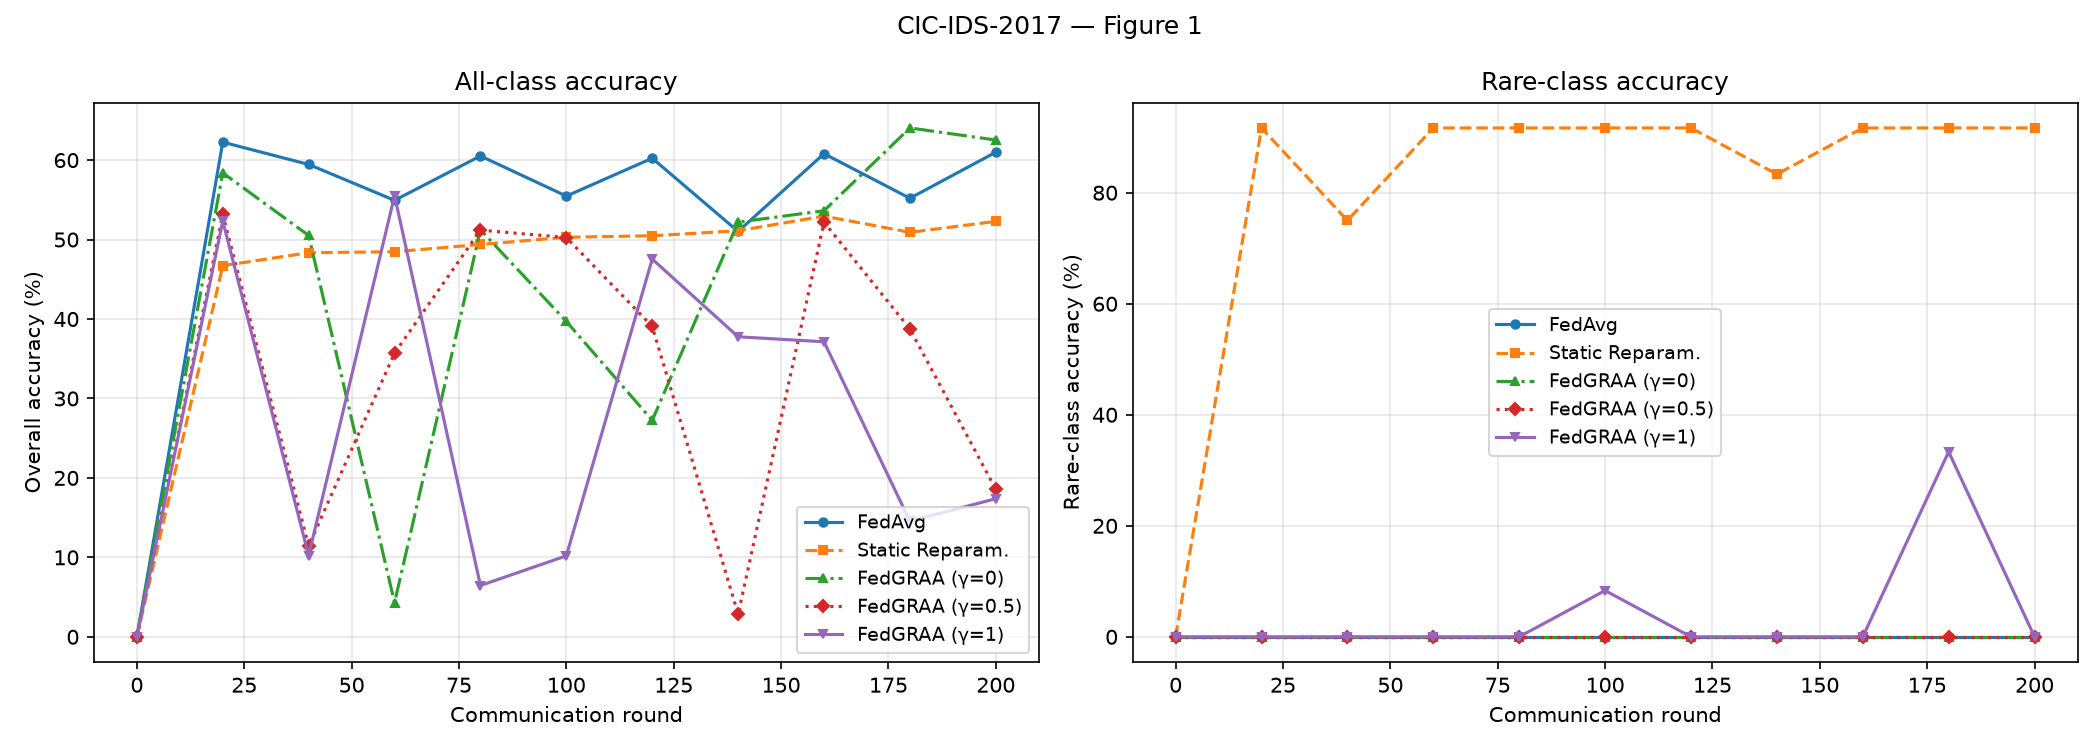
\includegraphics[width=0.74\textwidth]{figures/CIC-IDS-2017_figure1.png}
    \caption{CIC-IDS-2017.}
    \label{fig:cic-gamma-sweep}
  \end{subfigure}\\[4pt]
  \begin{subfigure}[b]{\textwidth}
    \centering
    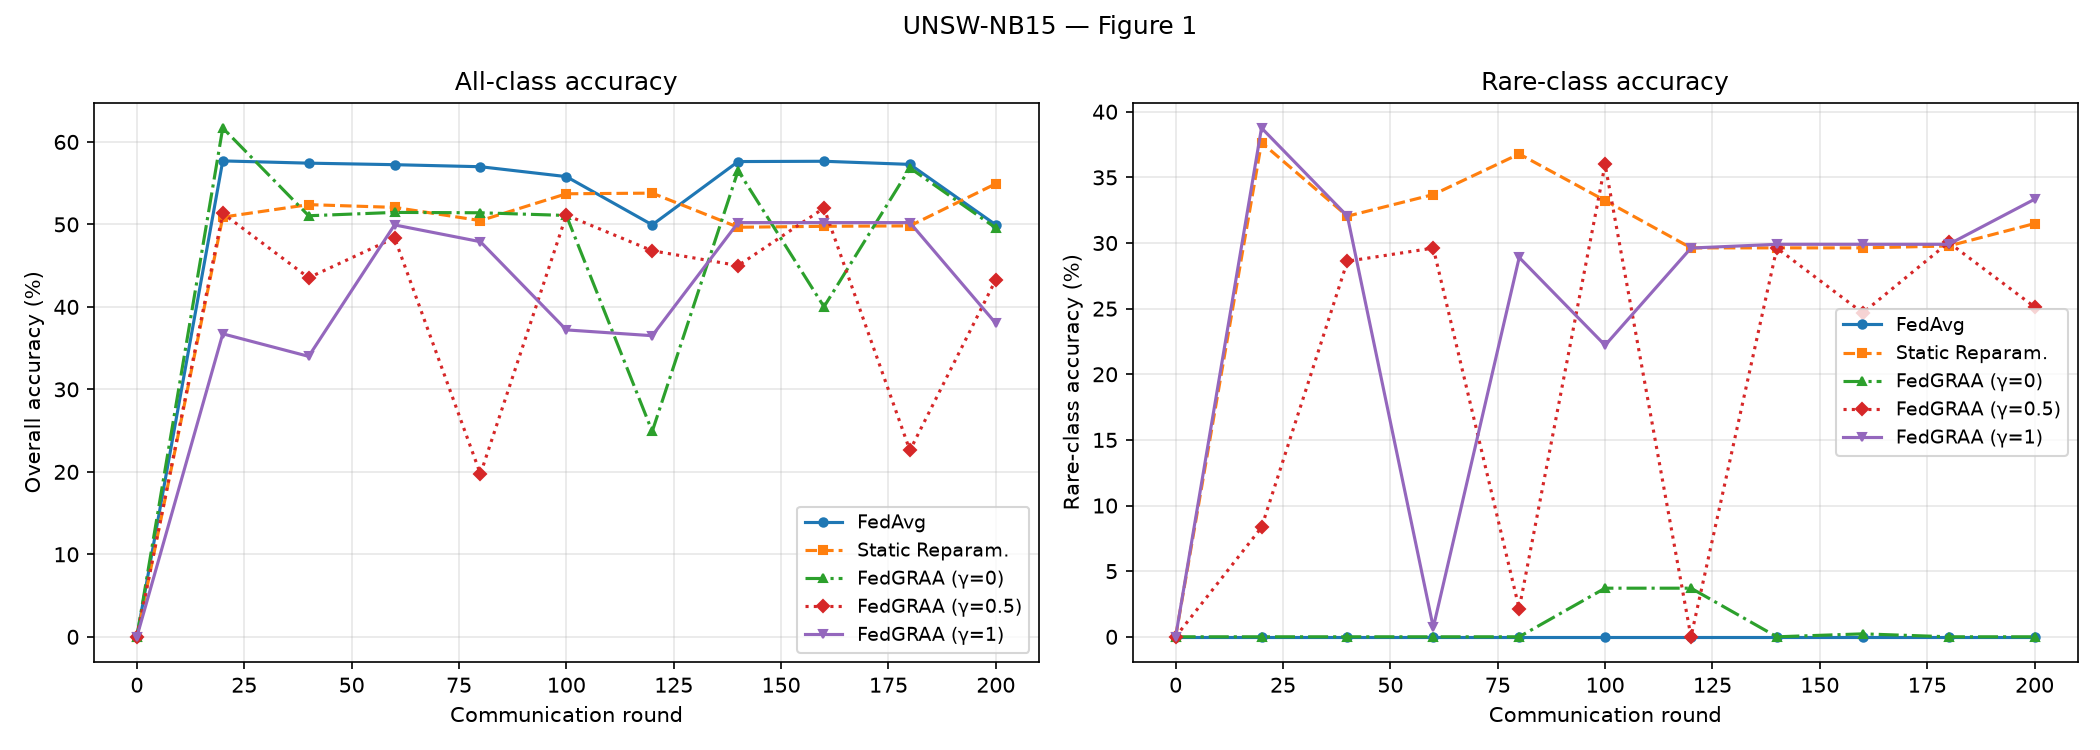
\includegraphics[width=0.74\textwidth]{figures/UNSW-NB15_figure1.png}
    \caption{UNSW-NB15.}
    \label{fig:unsw-gamma-sweep}
  \end{subfigure}
  \caption{200-round $\gamma$ sweeps (Stage A, seed 0): all-class accuracy,
  rare-class accuracy and composite loss for FedAvg, static
  reparameterization and literal FedGRAA at $\gamma \in \{0, 0.5, 1\}$. On
  UNSW (b) the literal $\gamma = 1$ arm nominally exceeds the paper's
  printed claim yet diverges in composite loss.}
  \label{fig:gamma-sweeps}
\end{figure}

\begin{table}[htbp]
  \centering
  \caption{Stage A $\gamma$ sweep, final round (seed 0, $n = 3$). Composite
  loss is reported for FedGRAA arms only.}
  \label{tab:stagea-sweep}
  \footnotesize
  \begin{tabular}{@{}llll@{}}
    \toprule
    Method & All-class acc.\ & Rare-class acc.\ & Final loss \\
    \midrule
    \multicolumn{4}{@{}l}{\emph{CIC-IDS-2017}}\\
    FedAvg            & 60.997\% & 0.00\% & -- \\
    Static reparam.\  & 52.290\% & 91.67\% & -- \\
    FedGRAA $\gamma=0$   & 62.526\% & 0.00\% & 94{,}909.25 \\
    FedGRAA $\gamma=0.5$ & 18.560\% & 0.00\% & 2.71 (peak 5.03) \\
    FedGRAA $\gamma=1$   & 17.384\% & 0.00\% & 3.14 (peak 58.41) \\
    \midrule
    \multicolumn{4}{@{}l}{\emph{UNSW-NB15}}\\
    FedAvg            & 49.947\% & 0.00\% & -- \\
    Static reparam.\  & 54.930\% & 31.48\% & -- \\
    FedGRAA $\gamma=0$   & 49.577\% & 0.00\% & 0.798 \\
    FedGRAA $\gamma=0.5$ & 43.297\% & 25.13\% & 1.524 \\
    FedGRAA $\gamma=1$   & 38.005\% & 33.33\% & 29{,}442.95 \\
    \bottomrule
  \end{tabular}
\end{table}

The $n$ sweeps (Figure~\ref{fig:nsweeps}) reinforce the diagnosis. On
CIC-IDS-2017 the literal composite loss reaches $8.03 \times 10^{15}$
($n{=}5$, $\gamma{=}0$), $1.72 \times 10^{18}$ ($n{=}5$, $\gamma{=}0.5$),
$2.04 \times 10^{15}$ ($n{=}5$, $\gamma{=}1$) and $2.81 \times 10^{16}$
($n{=}7$, $\gamma{=}0$) before collapsing. On UNSW-NB15 the $n = 7$
configuration is infeasible under the dataset's own taxonomy: only five
non-frequency-capped attack classes exist, so \texttt{rare\_client\_ids(7)}
truncates to the same five clients as $n = 5$ and the two panels are
metrically identical (maximum elementwise difference exactly zero) - an
honest divergence, preserved rather than patched, that independently
invalidates the paper's claimed UNSW $n = 7$ sweep.

\begin{figure}[htbp]
  \centering
  \begin{subfigure}[b]{\textwidth}
    \centering
    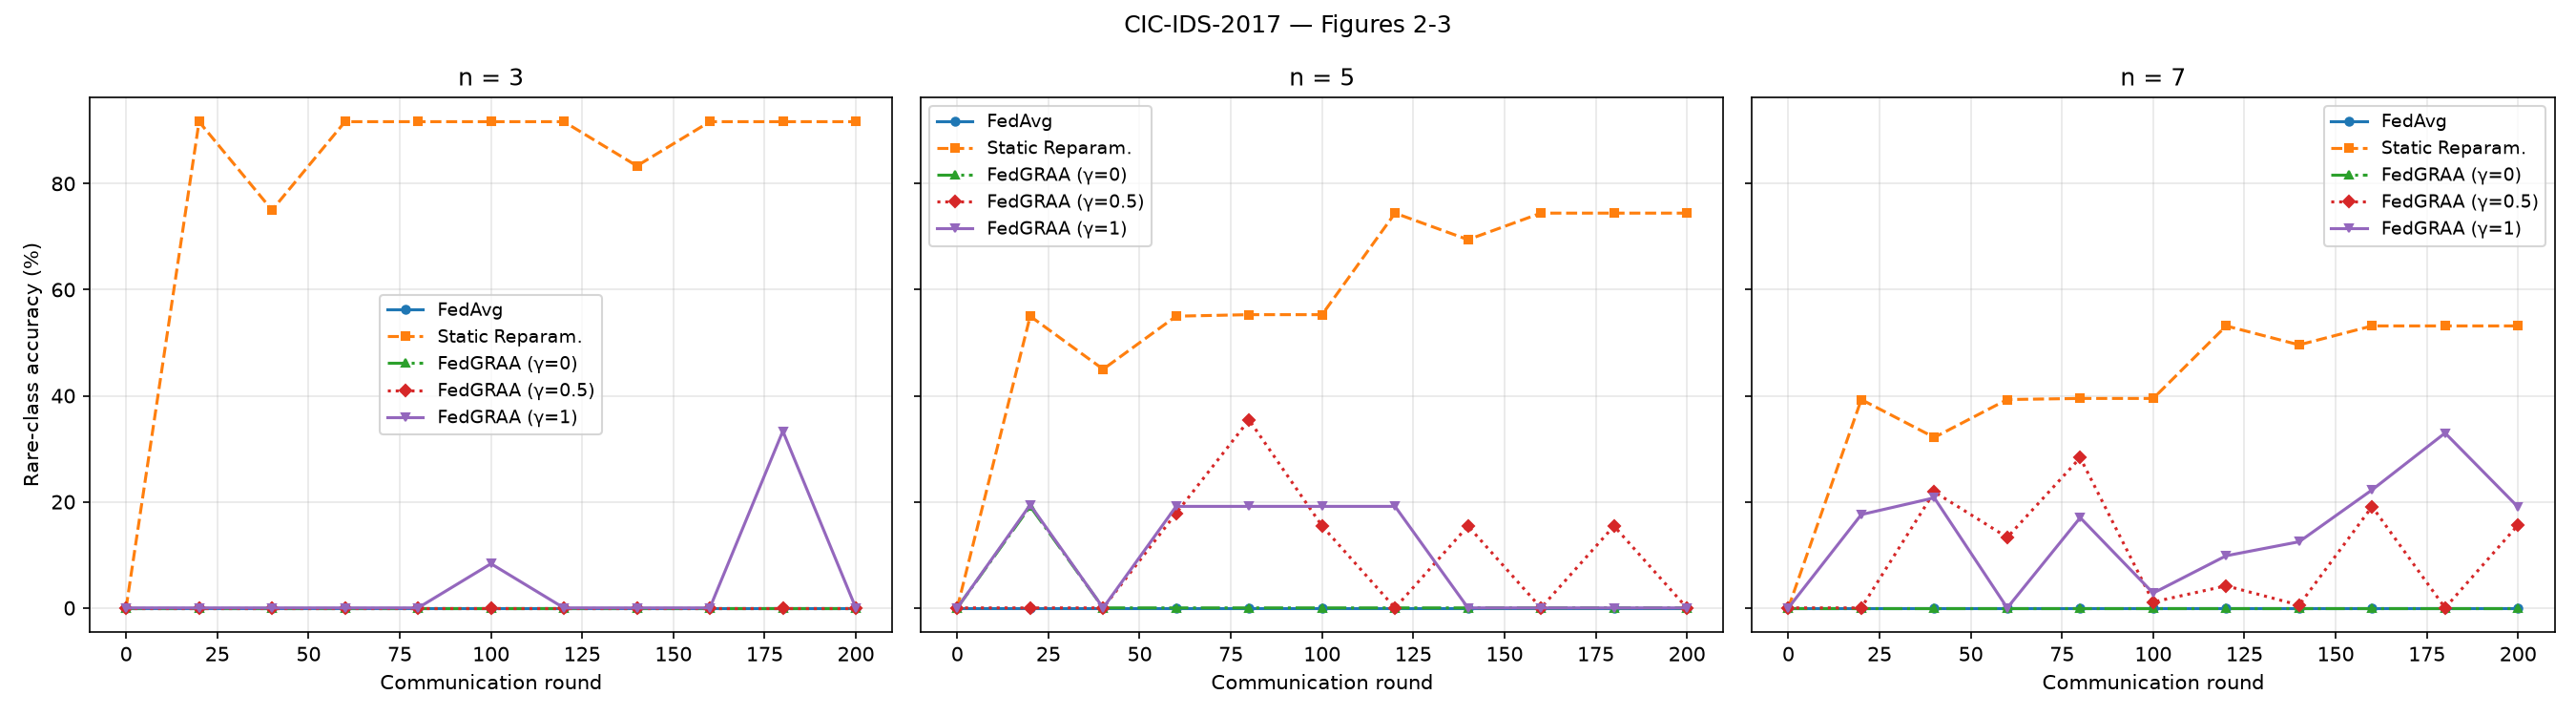
\includegraphics[width=0.74\textwidth]{figures/CIC-IDS-2017_figure2_3.png}
    \caption{CIC-IDS-2017.}
    \label{fig:cic-nsweep}
  \end{subfigure}\\[4pt]
  \begin{subfigure}[b]{\textwidth}
    \centering
    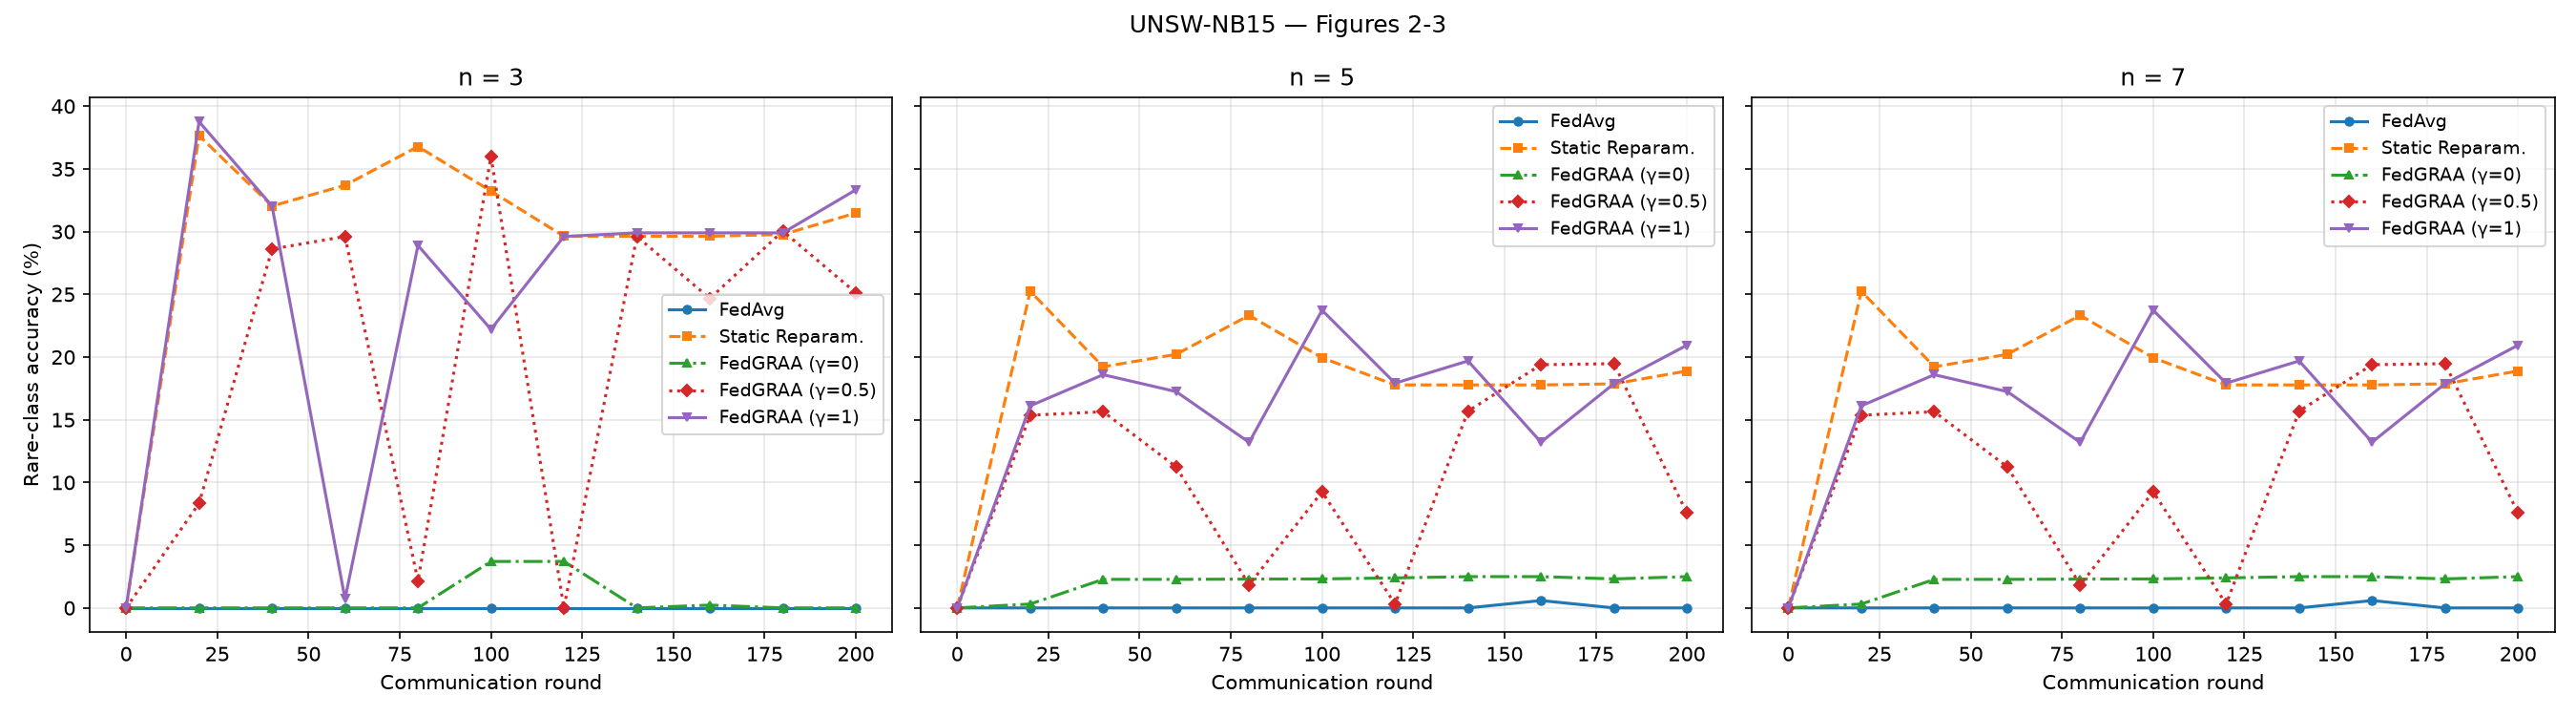
\includegraphics[width=0.74\textwidth]{figures/UNSW-NB15_figure2_3.png}
    \caption{UNSW-NB15.}
    \label{fig:unsw-nsweep}
  \end{subfigure}
  \caption{$n$ sweeps ($n \in \{3, 5, 7\}$, Stage A, seed 0). On CIC the
  literal composite loss blows up at every protection-set size, reaching
  $10^{18}$; on UNSW the $n = 7$ panel is metrically identical to $n = 5$
  because only five non-capped rare classes exist in the dataset.}
  \label{fig:nsweeps}
\end{figure}

A 60-round diagnostic pass recorded the weight vector directly
(Table~\ref{tab:literal-diagnostic}). In every cell, the first simplex
violation occurs at round~1: the iterate leaves $\Delta$ immediately and
never returns. Within 60 rounds $\sum_k w_k$ ranges from $-1.8915$ to
$+1.9596$ and individual coordinates reach $-0.75$.

\begin{table}[htbp]
  \centering
  \caption{Literal-arm diagnostic after 60 rounds (Stage A, seed 0):
  blowup ratio, terminal $\sum_k w_k$ and $\min_k w_k$. Every cell's first
  simplex violation is at round 1.}
  \label{tab:literal-diagnostic}
  \footnotesize
  \begin{tabular}{@{}lllll@{}}
    \toprule
    Dataset & $\gamma$ & Blowup & $\sum_k w_k$ & $\min_k w_k$ \\
    \midrule
    CIC & 0.0 & 3.8$\times$  & $-0.1155$ & $-0.2555$ \\
    CIC & 0.5 & 2.7$\times$  & $+0.4300$ & $-0.3203$ \\
    CIC & 1.0 & 193$\times$  & $-1.8915$ & $-0.7524$ \\
    UNSW & 0.0 & 1.3$\times$ & $+1.2727$ & $-0.3803$ \\
    UNSW & 0.5 & 1.2$\times$ & $-0.7312$ & $-0.4427$ \\
    UNSW & 1.0 & 7.6$\times$ & $+1.9596$ & $-0.2802$ \\
    \bottomrule
  \end{tabular}
\end{table}

\section{Diagnosis: the missing projection}
\label{sec:diagnosis}

Stage B converted the Stage A observation into a controlled experiment. Its
central empirical fact is stated precisely: across the 120 unprojected cells
of the factorial campaign (literal and $\eta'$-alone arms, 2 datasets
$\times$ 3 $\gamma$ $\times$ 10 seeds $\times$ 2 unprojected arms), the
weight iterate violates the simplex at round~1 in \textbf{120 out of 120}
cells, with zero exceptions; across the 120 projected cells the violation
count is \textbf{0}. Terminal $\sum_k w_k$ spans $[-2.621, +2.774]$ on CIC
and $[-1.869, +2.118]$ on UNSW, with $\min_k w_k$ reaching $-0.908$ and
$-1.157$ respectively; under projection the maximum observed
$|\sum_k w_k - 1|$ is $5.96 \times 10^{-8}$ (CIC) and $1.19 \times 10^{-7}$
(UNSW), i.e.\ float32 rounding noise.

Figure~\ref{fig:diag-loss} shows the mechanism in action on the CIC
$\gamma = 1$ seed-0 literal run: the composite loss trace $2.98 \to 2.77 \to
4.53 \to 6.06 \to 40.52 \to \dots \to 149.79$ (round 10), peaking at 574.44
at round 11, for a $192.99\times$ blowup - exactly the behaviour the paper's
Lemma~1
(monotone decrease) rules out - the lemma's premise $w \in \Delta$ fails,
so its conclusion fails. Once $w$ leaves the simplex, $\theta'_g =
\sum_k w_k \theta_k$ is an unbounded affine extrapolation rather than a
convex combination, and $\partial L'/\partial w$ feeds on a model outside
$\operatorname{conv}\{\theta_k\}$. The heaviest divergence is the CIC
$\gamma = 0$ seed-8 run, whose loss reaches 5{,}113{,}104 after a
$\sim$28-round quiescent period (blowup $1.86 \times 10^{6}$); the worst
UNSW literal cell reaches $46.85\times$. Figure~\ref{fig:diag-weights}
plots the weight trajectory on the same run.

\begin{figure}[htbp]
  \centering
  \begin{subfigure}[b]{0.49\textwidth}
    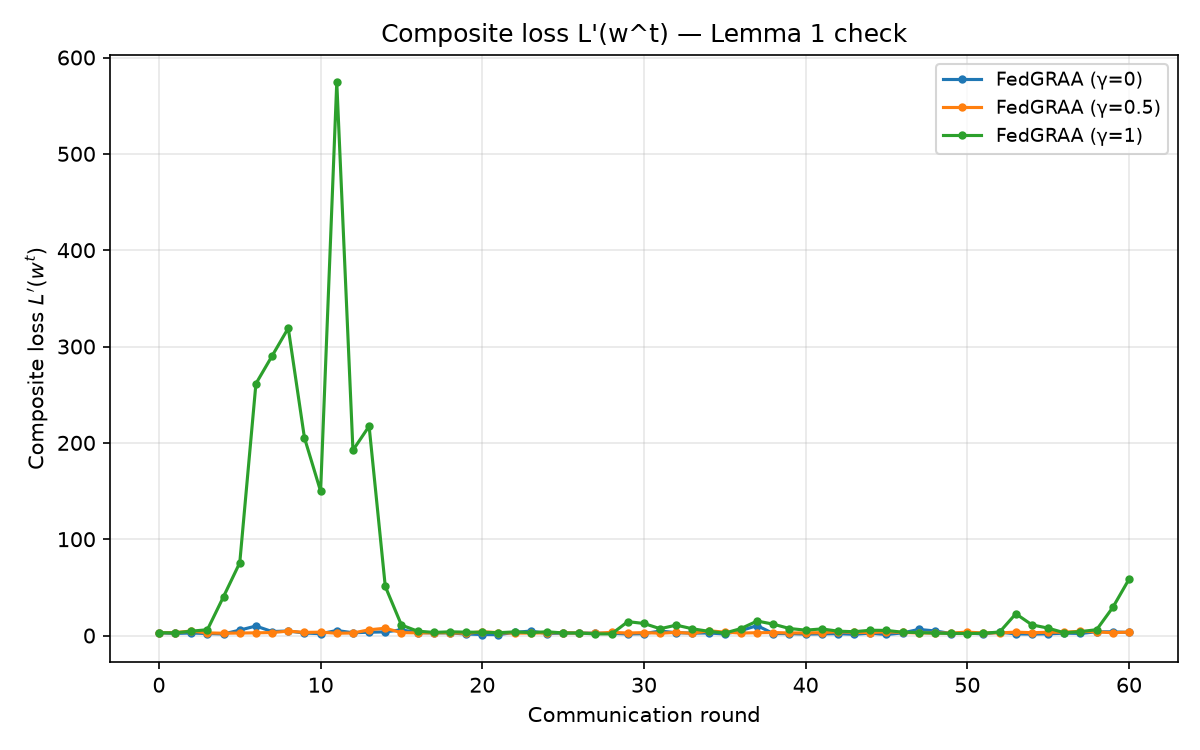
\includegraphics[width=0.74\textwidth]{figures/diagnosis_literal_composite_loss.png}
    \caption{Composite-loss traces diverge.}
    \label{fig:diag-loss}
  \end{subfigure}\hfill
  \begin{subfigure}[b]{0.49\textwidth}
    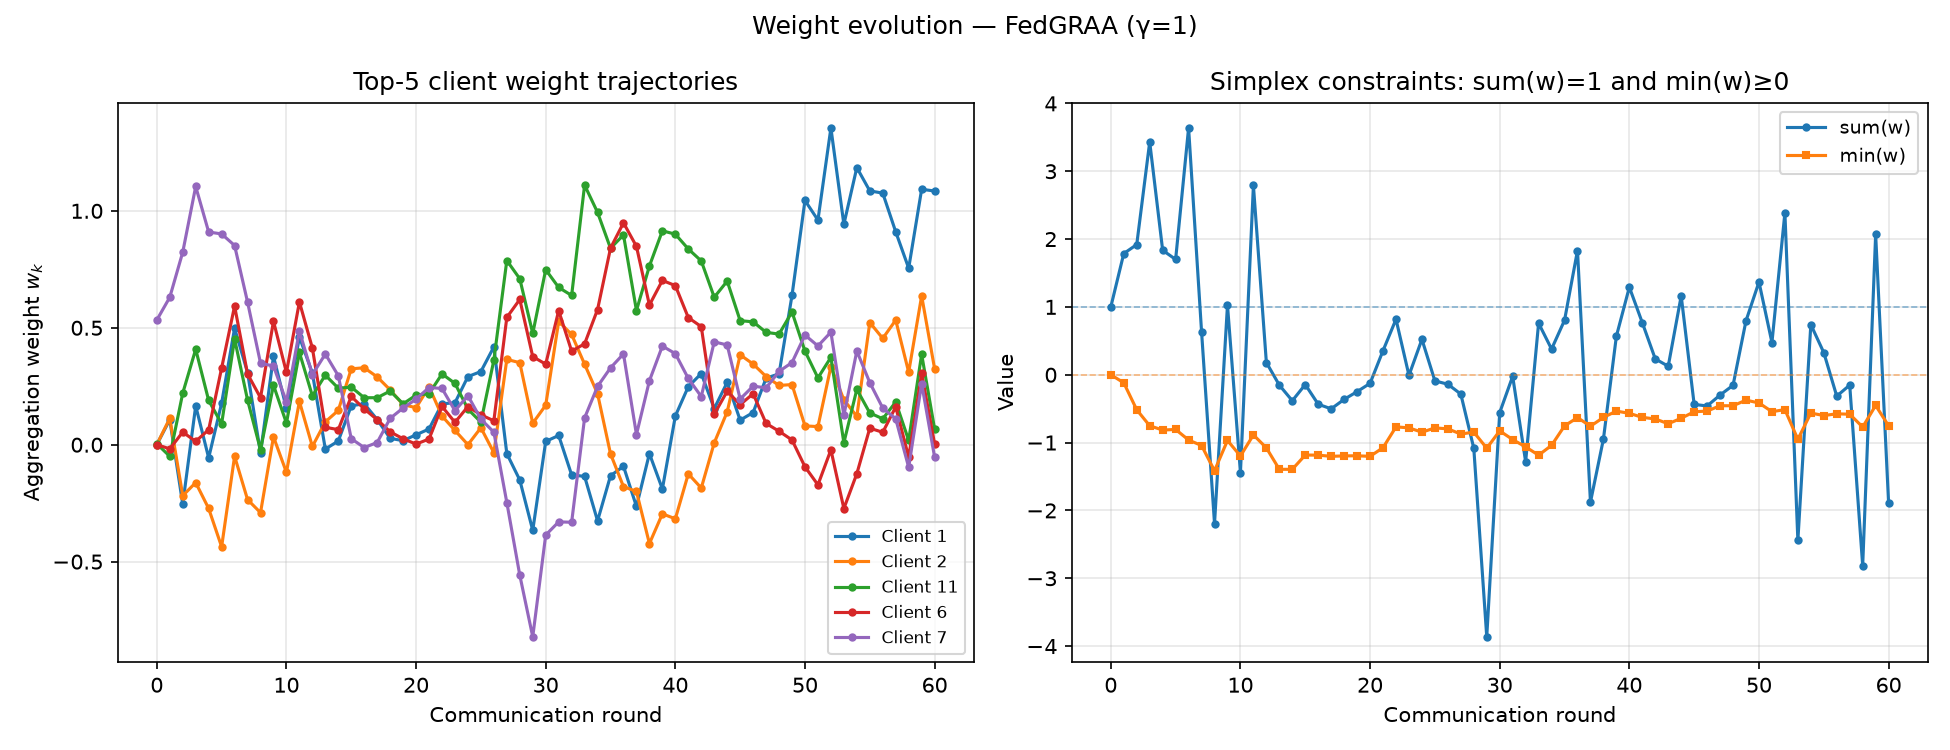
\includegraphics[width=0.74\textwidth]{figures/diagnosis_literal_weights_g1p0.png}
    \caption{Weights leave the simplex at round 1.}
    \label{fig:diag-weights}
  \end{subfigure}
  \caption{Literal-update diagnosis (CIC, $\gamma = 1$, seed 0): (a) the
  composite-loss trace diverges although Lemma 1 guarantees monotone
  decrease; (b) aggregation-weight coordinates leave $[0,1]$ and
  $\sum_k w_k$ leaves 1 at round 1 in every cell.}
  \label{fig:diagnosis}
\end{figure}

A subsidiary measurement worth reporting: the strict per-step reading of
Lemma~1 (the \texttt{monotone\_lemma1} field) holds in only 4 of 240
diagnostic cells - and is \emph{false} on every corrected cell, including
those with blowup exactly $1.00\times$, because the fix's loss can rebound
slightly after an initial monotone descent. The lemma as printed describes
a trajectory that essentially never occurs, in either direction.

\section{Stage B - the fix, statistically}
\label{sec:stageb}

The Stage B ablation (Table~\ref{tab:ablation},
Figures~\ref{fig:ablation-cic} and \ref{fig:ablation-unsw}) separates the
two candidate levers: projection onto $\Delta$, and the learning-rate cut
$\eta': 0.1 \to 0.01$. Three findings survive every comparison.

\begin{table}[htbp]
  \centering
  \caption{Stage B ablation on both datasets: rare-class recall mean [95\%
  bootstrap CI], all-class accuracy and composite-loss blowup (median;
  max), 10 seeds per cell. Stars mark Holm-corrected significance of each
  arm against \texttt{both} within a $\gamma$
  (${*}<.05$, ${*}{*}<.01$, ${*}{*}{*}<.001$).}
  \label{tab:ablation}
  \footnotesize
  \begin{tabular}{@{}llll@{}}
    \toprule
    Arm & $\gamma = 0$ & $\gamma = 0.5$ & $\gamma = 1$ \\
    \midrule
    \multicolumn{4}{@{}l}{\emph{CIC-IDS-2017}}\\
    FedAvg & 0.0\% [0.0, 0.0]${*}{*}{*}$ & 0.0\% [0.0, 0.0]${*}{*}{*}$ & 0.0\% [0.0, 0.0]${*}{*}{*}$ \\
     & \multicolumn{3}{l}{all-acc 55.7\%} \\
    Static reparam.\ & \multicolumn{3}{l}{84.4\% [77.2, 91.4] (all-acc 47.7\%; constant across $\gamma$; ${*}{*}$ vs \texttt{both} at $\gamma{=}0$)} \\
    Literal & 0.0\% [0.0, 0.0]${*}{*}{*}$ & 0.0\% [0.0, 0.0]${*}{*}{*}$ & 10.0\% [0.0, 30.0]${*}{*}{*}$ \\
     & all 48.9\%; 3.70$\times$/1.86e6$\times$ & all 26.7\%; 2.71$\times$/9.92$\times$ & all 32.9\%; 14.19$\times$/193$\times$ \\
    Proj.-alone & 0.0\% [0.0, 0.0]${*}{*}{*}$ & 0.0\% [0.0, 0.0]${*}{*}{*}$ & 51.0\% [24.2, 77.1] \\
     & all 59.8\%; 1.08$\times$/1.18$\times$ & all 54.8\%; 2.90$\times$/3.91$\times$ & all 48.4\%; 2.21$\times$/5.60$\times$ \\
    $\eta'$-alone & 27.5\% [12.5, 43.3]${*}{*}$ & 78.5\% [62.6, 92.2] & 88.9\% [68.9, 100.0] \\
     & all 71.7\%; 1.00$\times$ & all 44.1\%; 1.00$\times$ & all 15.2\%; 1.00$\times$/30.02$\times$ \\
    \textbf{Both (the fix)} & \textbf{69.7\%} [61.1, 78.9] & \textbf{81.1\%} [66.4, 92.2] & \textbf{89.3\%} [83.6, 94.6] \\
     & all 62.3\%; 1.00$\times$ & all 54.2\%; 1.00$\times$ & all 44.3\%; 1.00$\times$ \\
    \midrule
    \multicolumn{4}{@{}l}{\emph{UNSW-NB15}}\\
    FedAvg & 0.0\% [0.0, 0.0] & 0.0\% [0.0, 0.0]${*}{*}{*}$ & 0.0\% [0.0, 0.0]${*}{*}{*}$ \\
     & \multicolumn{3}{l}{all-acc 55.8\%} \\
    Static reparam.\ & \multicolumn{3}{l}{48.3\% [40.8, 56.0] (all-acc 52.7\%; constant across $\gamma$; ${*}{*}{*}$ at $\gamma{=}0$, ${*}{*}$ at $\gamma{=}1$ vs \texttt{both})} \\
    Literal & 0.1\% [0.0, 0.3] & 26.9\% [16.8, 36.2] & 27.6\% [15.0, 39.9]${*}{*}$ \\
     & all 54.9\%; 5.10$\times$/28.16$\times$ & all 49.6\%; 1.50$\times$/2.23$\times$ & all 29.1\%; 8.26$\times$/46.85$\times$ \\
    Proj.-alone & 6.4\% [0.0, 16.0] & 47.7\% [35.0, 57.6] & 67.2\% [59.6, 73.6] \\
     & all 59.4\%; 1.00$\times$ & all 53.6\%; 1.03$\times$/1.32$\times$ & all 51.8\%; 1.36$\times$/2.06$\times$ \\
    $\eta'$-alone & 3.4\% [0.4, 7.8] & 12.1\% [5.2, 19.6]${*}$ & 36.4\% [33.7, 39.8]${*}{*}{*}$ \\
     & all 59.7\%; 1.00$\times$ & all 49.2\%; 1.00$\times$/1.06$\times$ & all 13.3\%; 1.19$\times$/1.48$\times$ \\
    \textbf{Both (the fix)} & \textbf{1.7\%} [0.0, 4.6] & \textbf{37.1\%} [28.4, 45.7] & \textbf{69.2\%} [63.4, 73.8] \\
     & all 58.8\%; 1.00$\times$ & all 53.2\%; 1.03$\times$/1.39$\times$ & all 52.2\%; 1.32$\times$/1.87$\times$ \\
    \bottomrule
  \end{tabular}
\end{table}

\begin{figure}[htbp]
  \centering
  \begin{subfigure}[b]{\textwidth}
    \centering
    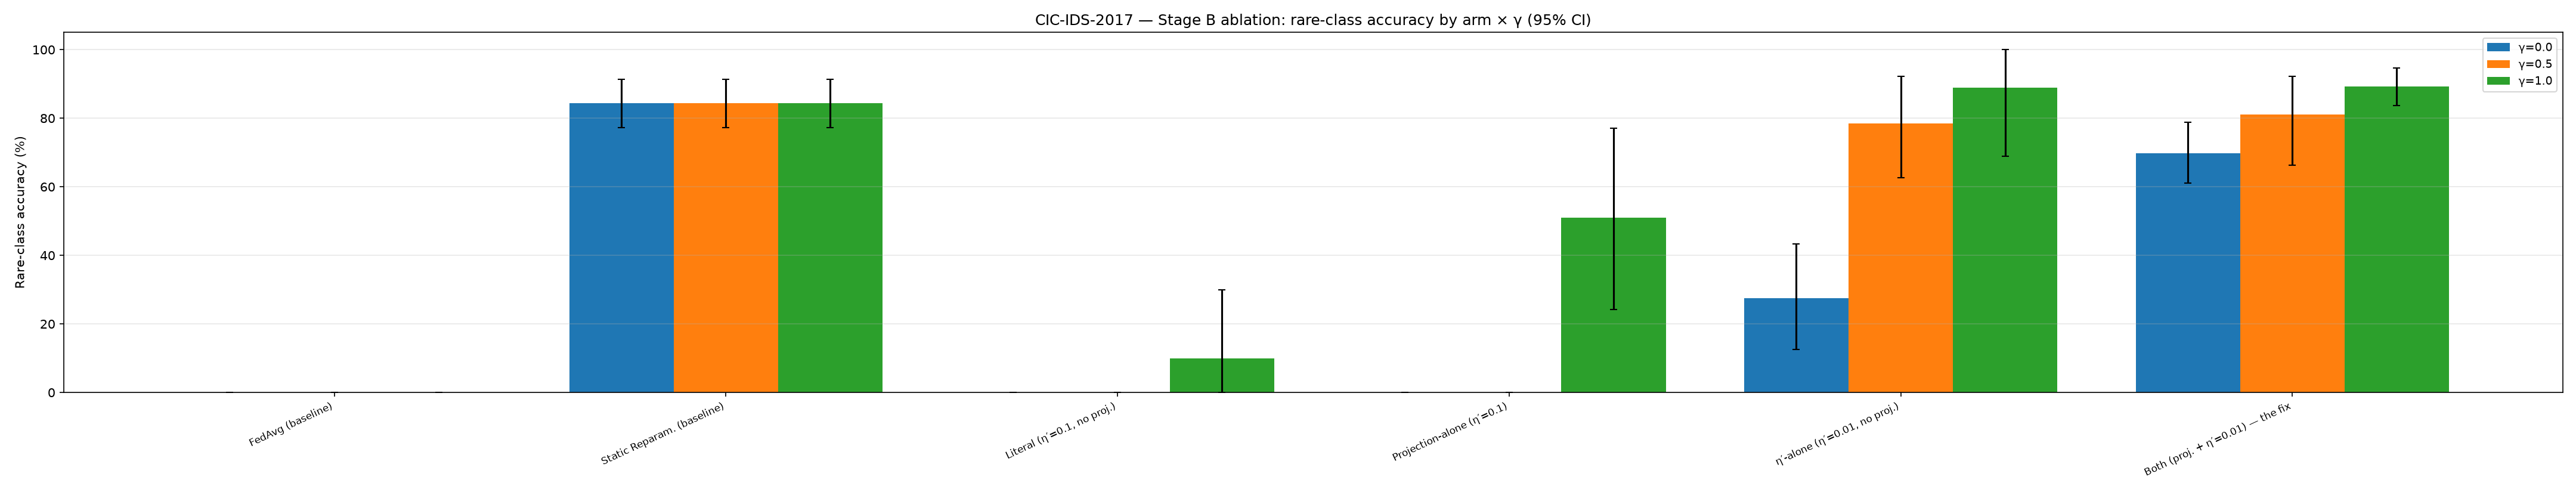
\includegraphics[width=0.74\textwidth]{figures/CIC_IDS_2017_ablation.png}
    \caption{CIC-IDS-2017.}
    \label{fig:ablation-cic}
  \end{subfigure}
  \begin{subfigure}[b]{\textwidth}
    \centering
    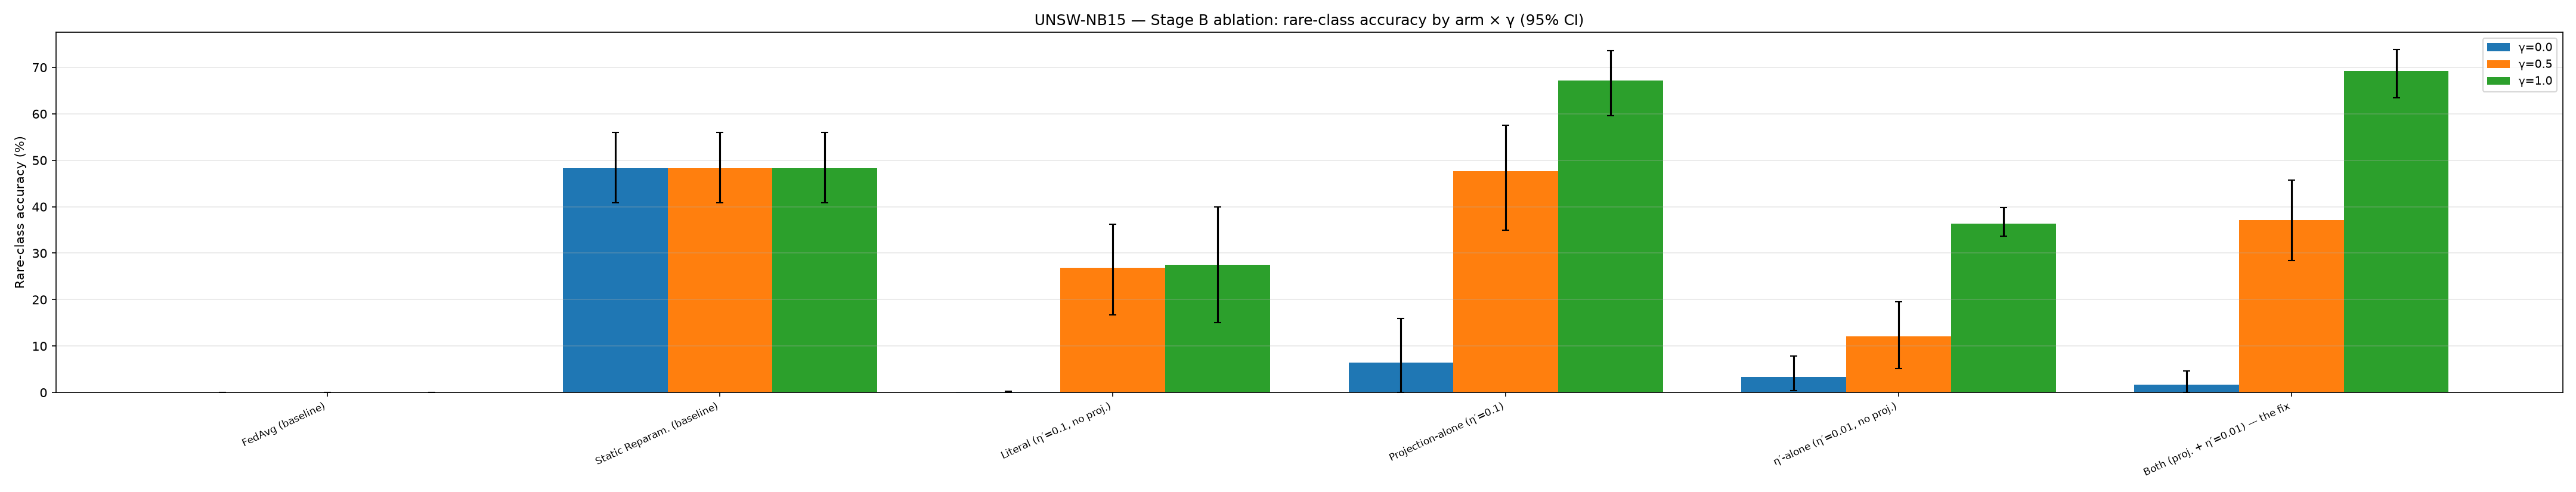
\includegraphics[width=0.74\textwidth]{figures/UNSW_NB15_ablation.png}
    \caption{UNSW-NB15.}
    \label{fig:ablation-unsw}
  \end{subfigure}
  \caption{Stage B factorial ablation on both datasets (10 seeds per cell).}
  \label{fig:ablation}
\end{figure}

First, feasibility is restored only by projection, and it is restored
completely: all 120 projected cells hold $w^t \in \Delta$ to float32
precision, while the $\eta'$ cut alone leaves every unprojected cell
violating at round~1. Projection is the structurally necessary,
dataset-independent lever.

Second, the lever that drives rare-class accuracy is dataset-dependent and
near-mirror-image (Table~\ref{tab:factorial}). On CIC the $\eta'$ cut
carries the recovery ($+48.6$ to $+79.8$ percentage points, versus
projection's $+1.3$ to $+21.1$); on UNSW the pattern inverts - projection
contributes $+22.9$ to $+36.2$ points at $\gamma \geq 0.5$ while the
$\eta'$ main effect is negligible or negative (a $-12.7$-point estimate at
$\gamma = 0.5$). The Stage~A preview's hypothesis that both levers are
always necessary is thereby refuted; what survives is a weaker but more
robust claim.

\begin{table}[htbp]
  \centering
  \caption{Factorial main effects on rare-class recall (percentage points,
  [95\% bootstrap CI]). The dominant lever differs by dataset.}
  \label{tab:factorial}
  \footnotesize
  \begin{tabular}{@{}lllll@{}}
    \toprule
    Dataset & $\gamma$ & Projection & $\eta'$ cut & Interaction \\
    \midrule
    CIC  & 0.0 & $+21.1$ [11.0, 31.7]  & $+48.6$ [41.1, 56.0]  & $+42.2$ [21.9, 63.3] \\
    CIC  & 0.5 & $+1.3$ [$-9.6$, 10.9] & $+79.8$ [70.1, 89.3]  & $+2.6$ [$-19.2$, 21.8] \\
    CIC  & 1.0 & $+20.7$ [5.3, 35.7]   & $+58.6$ [41.5, 75.0]  & $-40.6$ [$-75.8$, $-0.5$] \\
    UNSW & 0.0 & $+2.3$ [$-1.0$, 6.6]  & $-0.8$ [$-4.5$, 1.8]  & $-8.0$ [$-17.3$, $-0.7$] \\
    UNSW & 0.5 & $+22.9$ [12.6, 32.5]  & $-12.7$ [$-22.1$, $-1.1$] & $+4.3$ [$-10.3$, 18.1] \\
    UNSW & 1.0 & $+36.2$ [25.3, 46.3]  & $+5.4$ [$-1.5$, 12.5] & $-6.8$ [$-18.9$, 6.4] \\
    \bottomrule
  \end{tabular}
\end{table}

Third, \texttt{both} is the only arm that is never catastrophically wrong on
either metric, on either dataset, at any $\gamma$. The single-lever arms
each exhibit a failure mode: $\eta'$-alone collapses all-class accuracy to
15.2\% on CIC at $\gamma = 1$ (29 points below \texttt{both}), and
projection-alone reaches only 51.0\% rare-class recall there (38 points
below). The dual-metric requirement matters concretely: on CIC at
$\gamma = 1$, $\eta'$-alone \emph{ties} \texttt{both} on rare-class recall
(88.9\% versus 89.3\%, Holm $p = 0.97$) while sitting at 15.2\% all-class
accuracy versus 44.3\% (Holm $p = 5.6 \times 10^{-4}$, Cohen's
$d = +1.99$) - a starvation pathology in which the weight learner has
concentrated all mass on the rare-class clients. An arm that matches the fix
on the headline metric while collapsing the secondary one has not matched
the fix. Per-seed, the fix's blowup is strictly lower than the literal
arm's in 59 of 60 cells (one tie), and its rare-class recall is strictly
higher in 29/30 CIC cells and 19/30 UNSW cells. The eleven UNSW cells where
the fix does not strictly win sit at $\gamma \le 0.5$ - eight at the
pathological $\gamma = 0$ (two literal wins, six zero-ties, where optimizing
only the non-protected strata suppresses the protected ones) and three
literal wins at $\gamma = 0.5$; the single CIC loss is instead at
$\gamma = 1$ - the regime the manuscript's headline claim lives in - where
the fix beats the literal arm on rare-class recall on 10/10 UNSW seeds and
9/10 CIC seeds, that loss being the anomalous seed-6 literal run that
happened not to diverge; on all-class accuracy it wins 10/10 on UNSW and
6/10 on CIC.

The literal arm's UNSW failure mode deserves emphasis because it is a
\emph{variance} failure rather than a consistent zero: at $\gamma = 0.5$
the ten seeds' rare-class recalls are 29.6, 42.8, 0.4, 43.3, 44.0, 38.5,
3.4, 31.0, 24.2 and 11.8 per cent - a spread of 0.4\% to 44.0\% that no
single-seed reproduction could have detected. This is the sharpest
evidence that the published algorithm's behaviour is seed-unstable even
when its mean is nonzero.

\section{Stage C - the FedGRAA-v2 frontier}
\label{sec:stagec}

Stage C evaluates the privacy-compliant redesign against 19 external
baselines on the identical harness: three data-free contribution estimators
(CELM, SpectralFed, CoAst), three trust-based robust aggregators (FLTrust,
RAGA, FedTruth), eight NIDS-specific or adaptive methods (FedMADE,
SBFedNIDS, FedAPA, FedAWA, DA-PFL, FedAWARE, AdaAggRL, FedPGO) and five
classic optimizers (FedAvg, FedProx, FedOpt, SCAFFOLD, FedNova - the last
two built from scratch). Table~\ref{tab:frontier} and
Figure~\ref{fig:frontier} summarize the frontier;
Figure~\ref{fig:classic-fl} isolates the classic-optimizer comparison.

\begin{figure}[htbp]
  \centering
  \begin{subfigure}[b]{\textwidth}
    \centering
    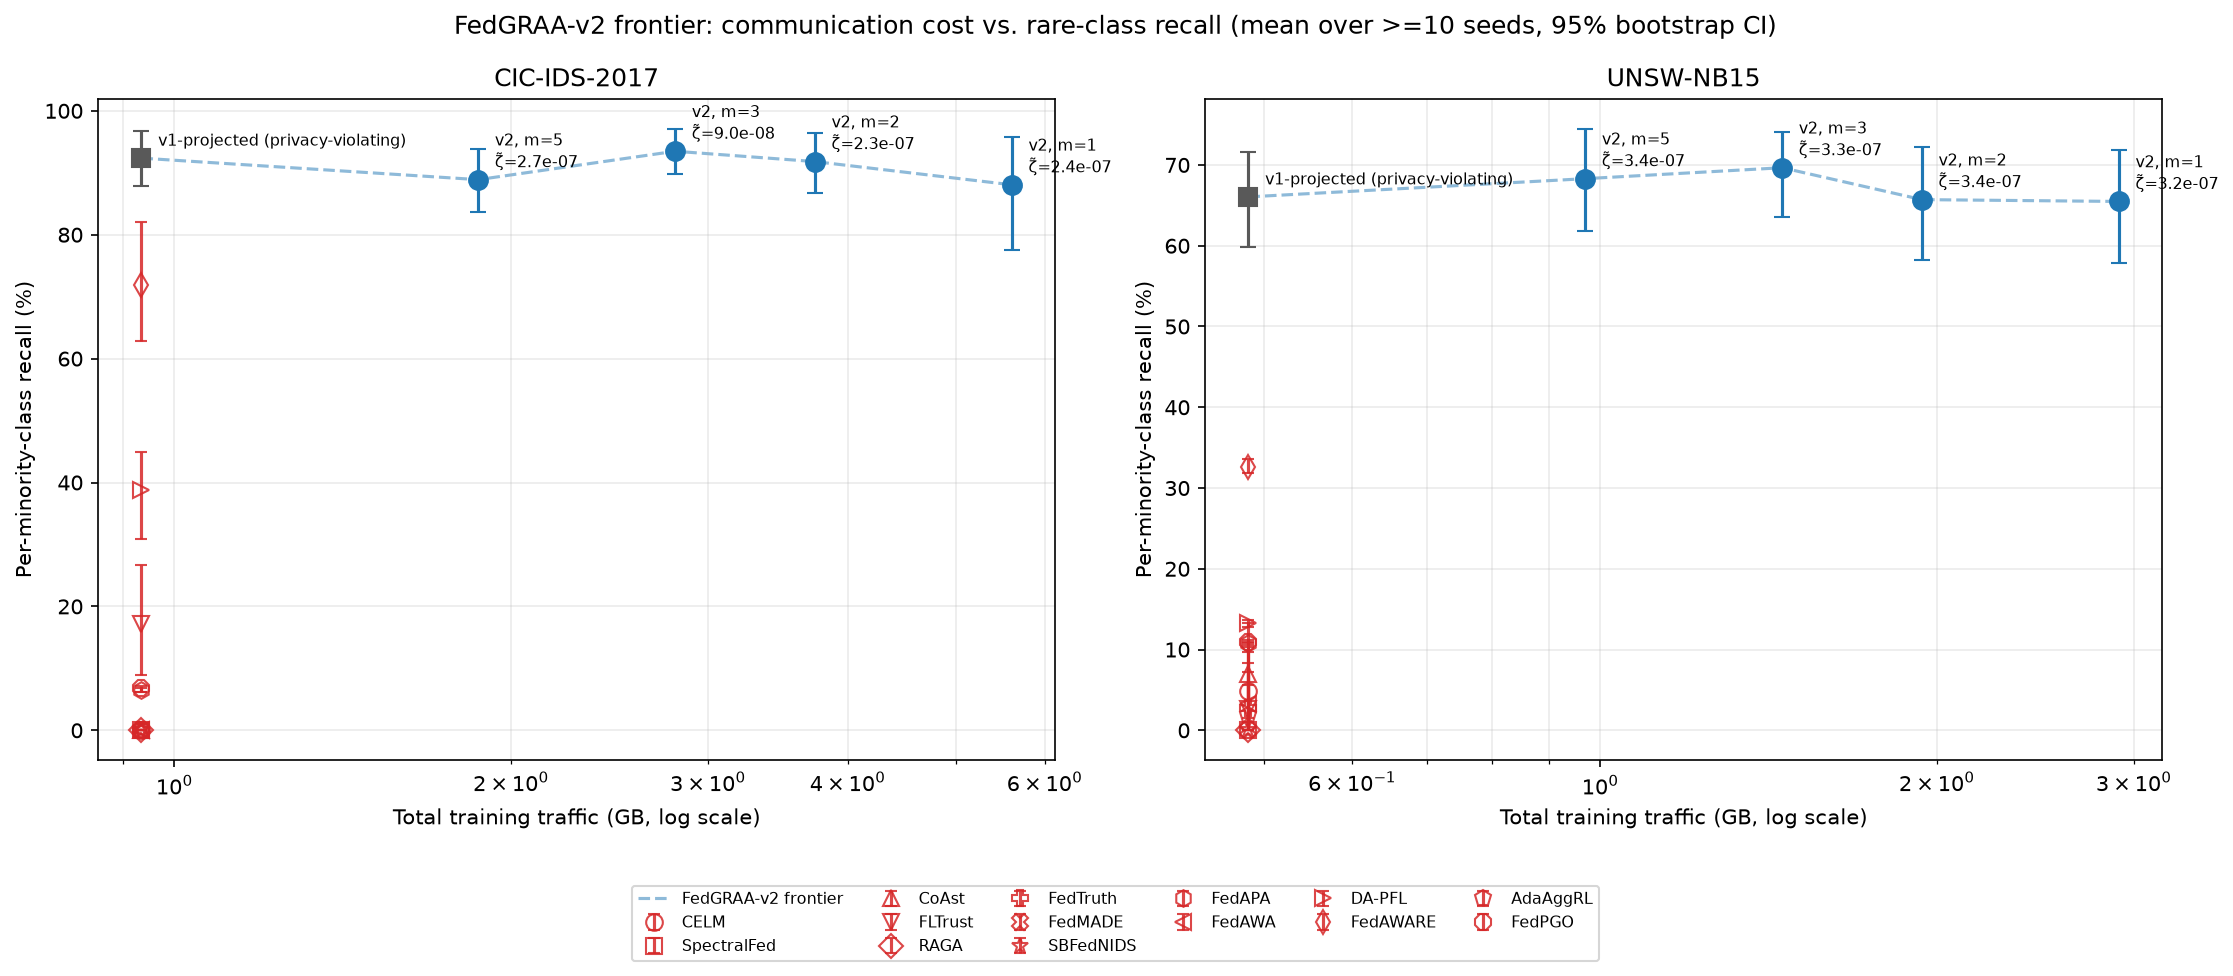
\includegraphics[width=0.74\textwidth]{figures/frontier_figure.png}
    \caption{Frontier: rare-class recall versus total training traffic.}
    \label{fig:frontier}
  \end{subfigure}
  \begin{subfigure}[b]{\textwidth}
    \centering
    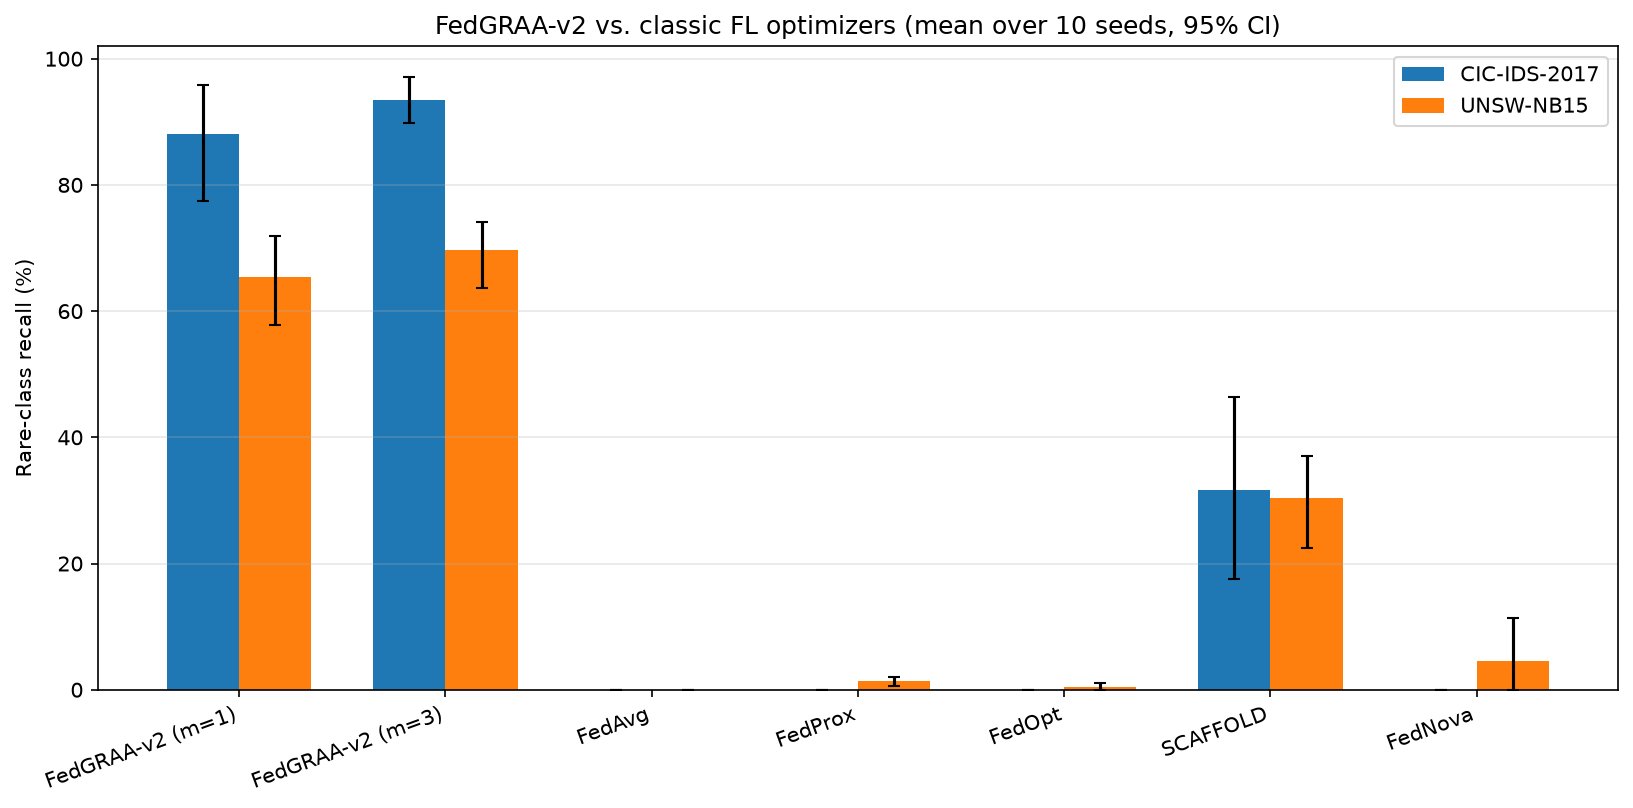
\includegraphics[width=0.74\textwidth]{figures/classic_fl_comparison.png}
    \caption{Against the five classic federated optimizers.}
    \label{fig:classic-fl}
  \end{subfigure}
  \caption{Stage C frontier for FedGRAA-v2 at $m \in \{1,2,3,5\}$ against 19
  baselines on both datasets.}
  \label{fig:stagec-frontier}
\end{figure}

\begin{table}[htbp]
  \centering
  \caption{Stage C frontier (selected arms): rare-class recall mean [95\%
  bootstrap CI], all-class accuracy and median total training traffic.
  The v1-projected arm is the privacy-violating oracle reference.}
  \label{tab:frontier}
  \footnotesize
  \begin{tabular}{@{}lllll@{}}
    \toprule
    Arm & GB & Rare recall [CI] & All-class & $\tilde{\zeta}$ \\
    \midrule
    \multicolumn{5}{@{}l}{\emph{CIC-IDS-2017}}\\
    v1-projected (oracle) & 0.934 & 92.36\% [87.92, 96.67] & 44.67\% & -- \\
    \textbf{v2, $m=3$} & 2.804 & \textbf{93.47\%} [89.86, 97.08] & 45.55\% & $9.0{\times}10^{-8}$ \\
    v2, $m=1$ & 5.607 & 88.06\% [77.50, 95.83] & 45.26\% & $2.4{\times}10^{-7}$ \\
    v2, $m=2$ & 3.738 & 91.81\% [86.67, 96.39] & 45.04\% & $2.3{\times}10^{-7}$ \\
    v2, $m=5$ & 1.869 & 88.89\% [83.61, 93.89] & 46.19\% & $2.8{\times}10^{-7}$ \\
    FedAWARE & 0.934 & 71.81\% [62.92, 82.08] & 42.56\% & -- \\
    DA-PFL & 0.934 & 38.77\% [30.83, 44.96] & 71.46\% & -- \\
    SCAFFOLD & 0.934 & 31.67\% [17.50, 46.39] & 30.04\% & -- \\
    FLTrust & 0.934 & 17.22\% [8.89, 26.67] & 70.50\% & -- \\
    FedPGO & 0.934 & 6.76\% [6.22, 7.14] & 51.45\% & -- \\
    FedAvg / FedProx / FedOpt / FedNova & 0.934 & 0.00\% each & 54.9--81.3\% & -- \\
    10 further baselines & 0.934 & $\le$ 6.58\% each (FedAPA) & -- & -- \\
    \midrule
    \multicolumn{5}{@{}l}{\emph{UNSW-NB15}}\\
    v1-projected (oracle) & 0.485 & 66.05\% [59.79, 71.57] & 52.24\% & -- \\
    \textbf{v2, $m=3$} & 1.454 & \textbf{69.66\%} [63.60, 74.12] & 52.24\% & $3.3{\times}10^{-7}$ \\
    v2, $m=1$ & 2.909 & 65.48\% [57.84, 71.89] & 52.21\% & $3.2{\times}10^{-7}$ \\
    v2, $m=2$ & 1.939 & 65.71\% [58.26, 72.24] & 52.25\% & $3.4{\times}10^{-7}$ \\
    v2, $m=5$ & 0.970 & 68.30\% [61.81, 74.47] & 52.18\% & $3.4{\times}10^{-7}$ \\
    FedAWARE & 0.485 & 32.65\% [31.80, 33.56] & 47.50\% & -- \\
    SCAFFOLD & 0.485 & 30.34\% [22.52, 36.97] & 45.78\% & -- \\
    DA-PFL & 0.485 & 13.25\% [12.81, 13.69] & 54.59\% & -- \\
    CoAst & 0.485 & 6.97\% [1.57, 13.25] & 53.83\% & -- \\
    FedNova & 0.485 & 4.62\% [0.00, 11.43] & 57.90\% & -- \\
    FedAvg / FedProx / FedOpt & 0.485 & $\le$ 1.33\% each & -- & -- \\
    11 further baselines & 0.485 & $\le$ 10.9\% each (FedPGO) & -- & -- \\
    \bottomrule
  \end{tabular}
\end{table}

Three observations follow. First, the privacy-compliant redesign is not
merely competitive with the oracle: at $m = 3$ it \emph{exceeds} the
privacy-violating v1-projected reference on both datasets (93.47\% versus
92.36\% on CIC; 69.66\% versus 66.05\% on UNSW), so removing the two
privacy assumptions cost no accuracy - the federated backward pass is, at
each refresh, algebraically identical to what a server-held $D_V$ would
compute, and the measured per-round gradient discrepancy $\tilde{\zeta}$
spans $9\times10^{-8}$ to $4\times10^{-7}$ across the frontier cells, below
the $10^{-6}$ exactness tolerance the test suite enforces. Second, the margin over the strongest external
baseline is large: FedAWARE, the best baseline on both datasets, trails the
best v2 arm by 21.7 points on CIC and 37.0 on UNSW. Third, every external
baseline sits strictly below the v2 frontier on both datasets, and most sit
at or near zero rare-class recall: the only baselines above 14\% anywhere
are FedAWARE, DA-PFL, SCAFFOLD, and FLTrust on CIC (17.22\%), while the
data-free contribution estimators (CELM, SpectralFed, CoAst) and the
trust-based aggregators RAGA and FedTruth collapse to 0--7\% - consistent
with the Section~\ref{sec:adaptive-agg} prediction that
anomaly-suppressing signals discard exactly the clients FedGRAA protects.

\section{Significance testing}
\label{sec:significance}

Every v2 arm was compared against every baseline with a paired Wilcoxon
signed-rank test over the 10 matched seeds, Holm-Bonferroni corrected within
each (dataset, refresh-interval) family of 14 comparisons: 112 comparisons
in total. \textbf{111 of 112 are significant} at $\alpha = 0.05$; the sole
exception is CIC v2\_m1 versus FedAWARE ($p_{\mathrm{holm}} = 0.0625$; v2
88.06\% versus 71.81\%), and the other three CIC refresh intervals clear
the same comparison at $p_{\mathrm{holm}} \leq 0.028$. Almost all
significant rows sit at the exact-test floor $p = 0.001953 = 2/2^{10}$,
the minimum attainable Wilcoxon $p$-value at $n = 10$ - a floor the report
states explicitly rather than implying stronger evidence than 10 seeds can
deliver. The count is reported as 111/112, not rounded up: the honest
summary is that the frontier margin is statistically supported everywhere
except a single cell, and that cell is the weakest v2 arm against the
strongest baseline. Table~\ref{tab:sig-perarm} gives the per-arm breakdown.

\begin{table}[htbp]
  \centering\footnotesize
  \caption{Significant Holm-corrected Wilcoxon comparisons per v2 arm
  (out of 14 baselines each). The single non-significant cell is CIC
  v2\_m1 vs.\ FedAWARE.}
  \label{tab:sig-perarm}
  \begin{tabular}{@{}lcccc@{}}
    \toprule
     & v2 $m{=}1$ & v2 $m{=}2$ & v2 $m{=}3$ & v2 $m{=}5$\\
    \midrule
    CIC-IDS-2017 & 13/14 & 14/14 & 14/14 & 14/14\\
    UNSW-NB15    & 14/14 & 14/14 & 14/14 & 14/14\\
    \bottomrule
  \end{tabular}
\end{table}

\section{Communication overhead}
\label{sec:overhead}

The two-phase protocol adds exactly one model-shaped array per client per
refresh (plus six scalars at Phase 1), so measured traffic follows the
closed form of Eq.~\eqref{eq:overhead}: $(1 + \lceil E'/m \rceil)\times$ the
plain FedAvg-shaped baseline, byte-exact to per-cell medians.
Table~\ref{tab:overhead} and Figure~\ref{fig:overhead} give the measured
values. The interesting operating point is $m = 3$: it halves the $m = 1$
communication cost (3.00$\times$ versus 6.00$\times$) while \emph{improving}
rare-class recall on both datasets (88.06\% $\to$ 93.47\% CIC; 65.48\%
$\to$ 69.66\% UNSW) - moderate staleness acts as an implicit regularizer on
the weight learner. The byte-exact values are those in
Table~\ref{tab:overhead}.

\begin{table}[htbp]
  \centering
  \caption{Measured communication overhead versus the FedAvg-shaped baseline
  ($E' = 5$ refreshes at $m = 1$): $(1 + \lceil E'/m \rceil)\times$,
  byte-exact.}
  \label{tab:overhead}
  \footnotesize
  \begin{tabular}{@{}lcccc@{}}
    \toprule
    & \multicolumn{2}{c}{CIC-IDS-2017} & \multicolumn{2}{c}{UNSW-NB15} \\
    \cmidrule(lr){2-3}\cmidrule(lr){4-5}
    Arm & GB & Ratio & GB & Ratio \\
    \midrule
    Baseline (all 19) & 0.934 & $1\times$ & 0.485 & $1\times$ \\
    v2, $m=1$ & 5.607 & $6.00\times$ & 2.909 & $6.00\times$ \\
    v2, $m=2$ & 3.738 & $4.00\times$ & 1.939 & $4.00\times$ \\
    v2, $m=3$ & 2.804 & $3.00\times$ & 1.454 & $3.00\times$ \\
    v2, $m=5$ & 1.869 & $2.00\times$ & 0.970 & $2.00\times$ \\
    \bottomrule
  \end{tabular}
\end{table}

\begin{figure}[htbp]
  \centering
  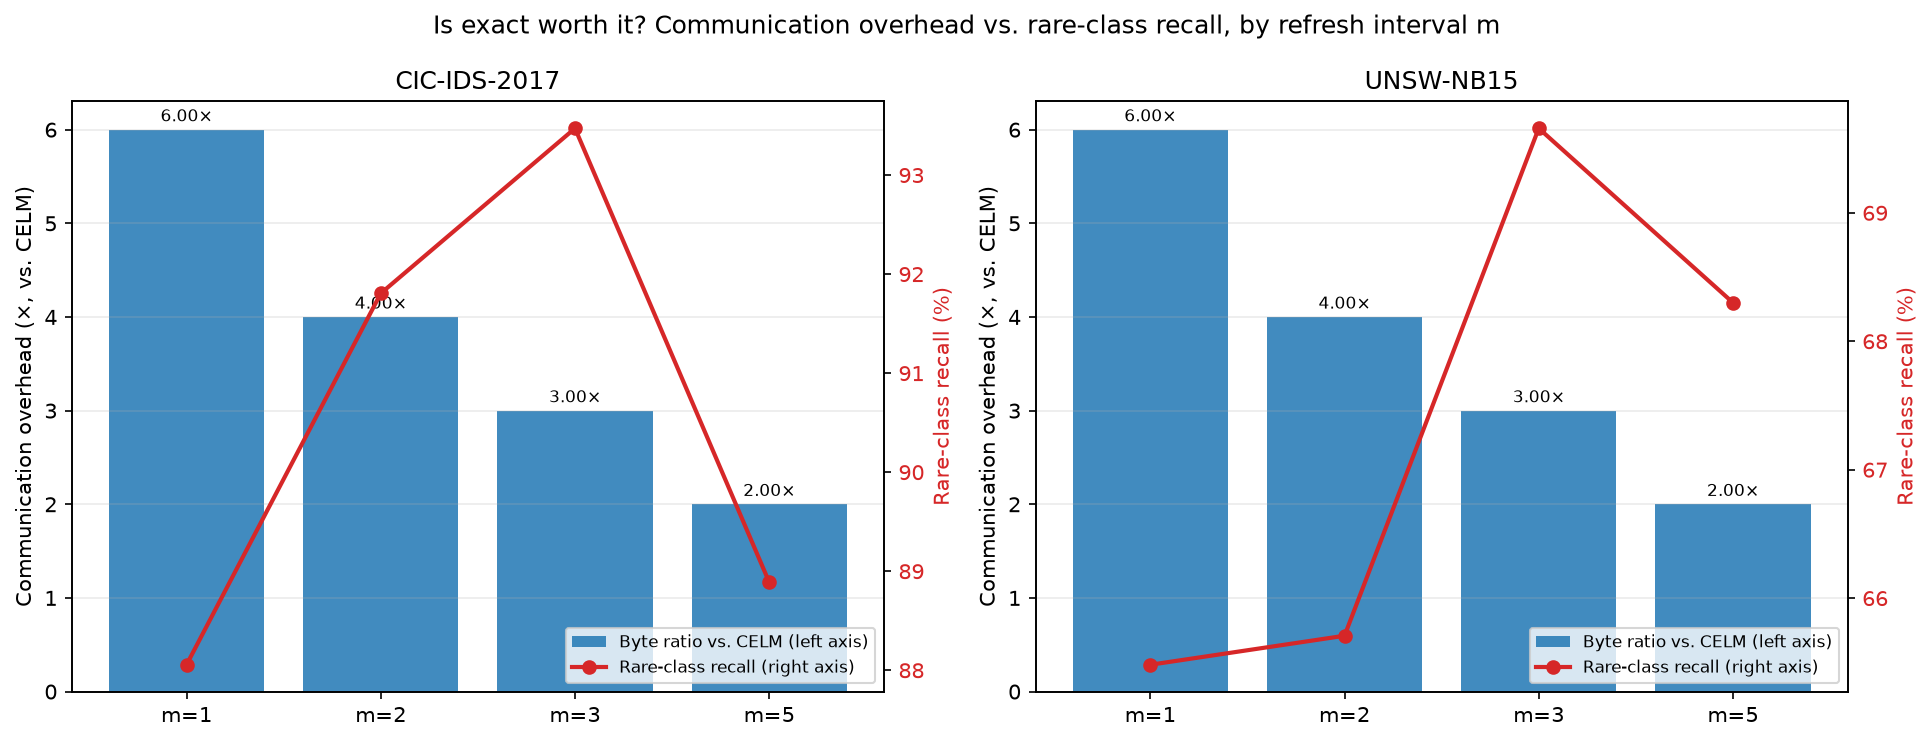
\includegraphics[width=0.62\textwidth]{figures/overhead_ratio.png}
  \caption{Communication overhead as a function of the refresh interval $m$,
  matching the closed form $(1 + \lceil E'/m \rceil)\times$.}
  \label{fig:overhead}
\end{figure}

\section{Adversarial robustness}
\label{sec:adversarial}

The T7/T7G campaigns measure what the Section~\ref{sec:attack-surface}
analysis predicts: an attacker who crafts its update to \emph{look like} a
rare-class contribution is up-weighted by construction. At 30\% attacker
fraction against undefended FedGRAA-v2, the mechanism-specific attack lifts
the mean per-attacker weight to \textbf{3.07$\times$} the uniform share on
CIC (0.219 versus $1/14 = 0.071$) and \textbf{2.71$\times$} on UNSW (0.301
versus $1/9 = 0.111$), sustained for $\sim$190 rounds
(Figure~\ref{fig:t7-weights}) - in several seeds the trajectory saturates at
exactly $1/n_{\mathrm{attackers}}$, i.e.\ all simplex mass on the attackers.

\begin{figure}[htbp]
  \centering
  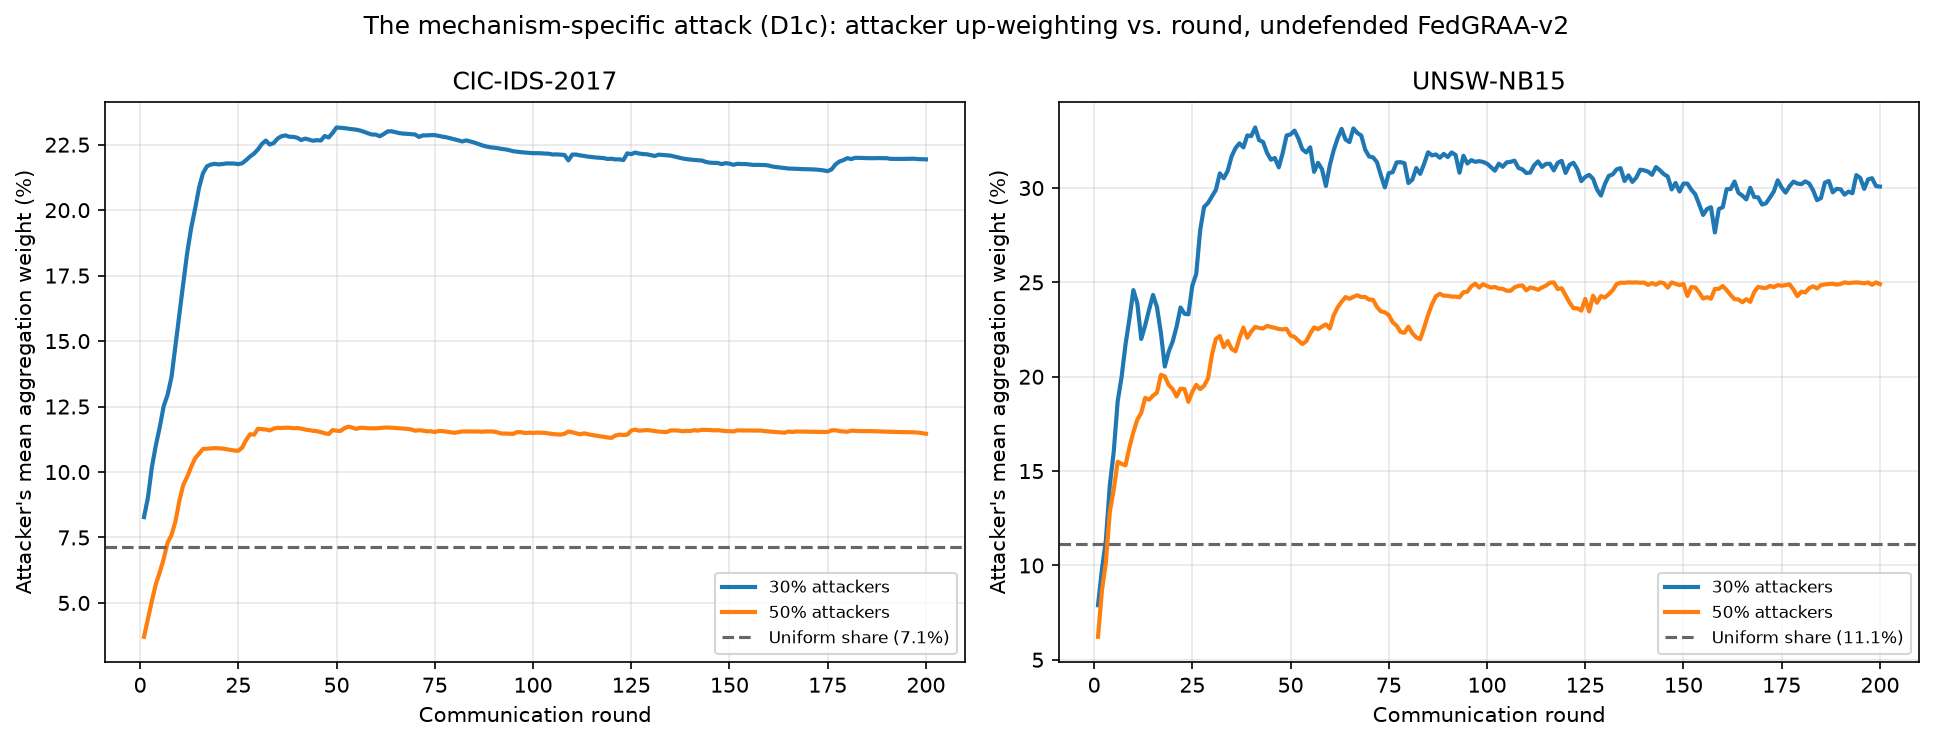
\includegraphics[width=0.74\textwidth]{figures/t7_attacker_weight_trajectory.png}
  \caption[Mean per-attacker aggregation weight under the rare-signature
  attack]{Mean per-attacker aggregation weight under the mechanism-specific
  rare-signature attack at 30\% attacker fraction, undefended FedGRAA-v2.
  The dashed lines mark the uniform share $1/K$ and the saturation cap
  $1/n_{\mathrm{attackers}}$.}
  \label{fig:t7-weights}
\end{figure}

The T7G $\gamma$ sweep (Table~\ref{tab:t7g}) refines the picture in two
directions. The up-weighting is \emph{non-monotonic} in $\gamma$, peaking at
$\gamma = 0.5$ in three of the four cells rather than at the most
rare-class-focused setting - the attack surface is largest when the
composite objective mixes protected and unprotected strata. And $\gamma = 0$
exhibits bimodal, coin-flip behaviour with an order-of-magnitude larger
seed variance ($\sigma$ 8--18$\times$ the $\gamma = 0.5$ value across the
four cells): individual seeds either
saturate the attackers' weight or leave it
near zero (UNSW 50\%, $\gamma = 0$: raw finals $[0.231, 0.208, 0.0, 0.0,
0.248]$, two seeds where the attack never took hold). At 50\% attacker
fraction the effect persists on UNSW (up to $2.24\times$) but weakens on
CIC, where the $\gamma = 1$ mean is $1.60\times$ and two of five seeds show
essentially no up-weighting - this corrects the manuscript draft's
``$2.0$-$2.2\times$'' prose, which the independent code-versus-paper audit
flagged as a transcription error.

\begin{table}[htbp]
  \centering
  \caption{T7G attacker-side $\gamma$ sweep: mean final attacker weight as a
  multiple of uniform per-client share (5 seeds; $\sigma$ = sample std of
  raw final weight). The attack surface peaks at $\gamma = 0.5$ in 3 of 4
  cells; $\gamma = 0$ is bimodal.}
  \label{tab:t7g}
  \footnotesize
  \begin{tabular}{@{}lllll@{}}
    \toprule
    Dataset & Attackers & $\gamma = 0$ & $\gamma = 0.5$ & $\gamma = 1$ \\
    \midrule
    CIC  & 30\% & $2.05\times$ ($\sigma$ 0.122) & \textbf{3.34$\times$} ($\sigma$ 0.007) & $3.07\times$ \\
    CIC  & 50\% & $0.93\times$ ($\sigma$ 0.068) & \textbf{1.82$\times$} ($\sigma$ 0.008) & $1.60\times$ \\
    UNSW & 30\% & $2.33\times$ ($\sigma$ 0.129) & \textbf{2.91$\times$} ($\sigma$ 0.010) & $2.71\times$ \\
    UNSW & 50\% & $1.24\times$ ($\sigma$ 0.126) & $2.11\times$ ($\sigma$ 0.012) & \textbf{2.24$\times$} \\
    \bottomrule
  \end{tabular}
\end{table}

Two external poisoning defenses were cross-evaluated against three attack
types (label-flip, pill-style model poisoning, and the adaptive attacker) at
30\% attacker fraction, 5 seeds per cell
(Table~\ref{tab:asr}, Figure~\ref{fig:t7-asr}). SecFedNIDS misses 53-75\% of
attacks on these datasets - a weak reproduction of its published
UNSW-NB15/CSE-CIC-IDS2018 evaluation, reported as such. WeiDetect is stronger on
the static attacks (0-20\% attack success rate) but the adaptive attacker
still reaches 60\% ASR on CIC.

\begin{table}[htbp]
  \centering
  \caption{T7 defense grid: attack success rate (ASR $= 1 -$ detection
  recall; lower is a better defense), 30\% attackers, 5 seeds.}
  \label{tab:asr}
  \footnotesize
  \begin{tabular}{@{}llll@{}}
    \toprule
    Defense & Attack & CIC ASR & UNSW ASR \\
    \midrule
    SecFedNIDS & label-flip    & 75.0\% & 60.0\% \\
    SecFedNIDS & model-poison  & 65.0\% & 60.0\% \\
    SecFedNIDS & adaptive      & 55.0\% & 53.3\% \\
    WeiDetect  & label-flip    & 15.0\% & 0.0\% \\
    WeiDetect  & model-poison  & 20.0\% & 6.7\% \\
    WeiDetect  & adaptive      & 60.0\% & 33.3\% \\
    \bottomrule
  \end{tabular}
\end{table}

\begin{figure}[htbp]
  \centering
  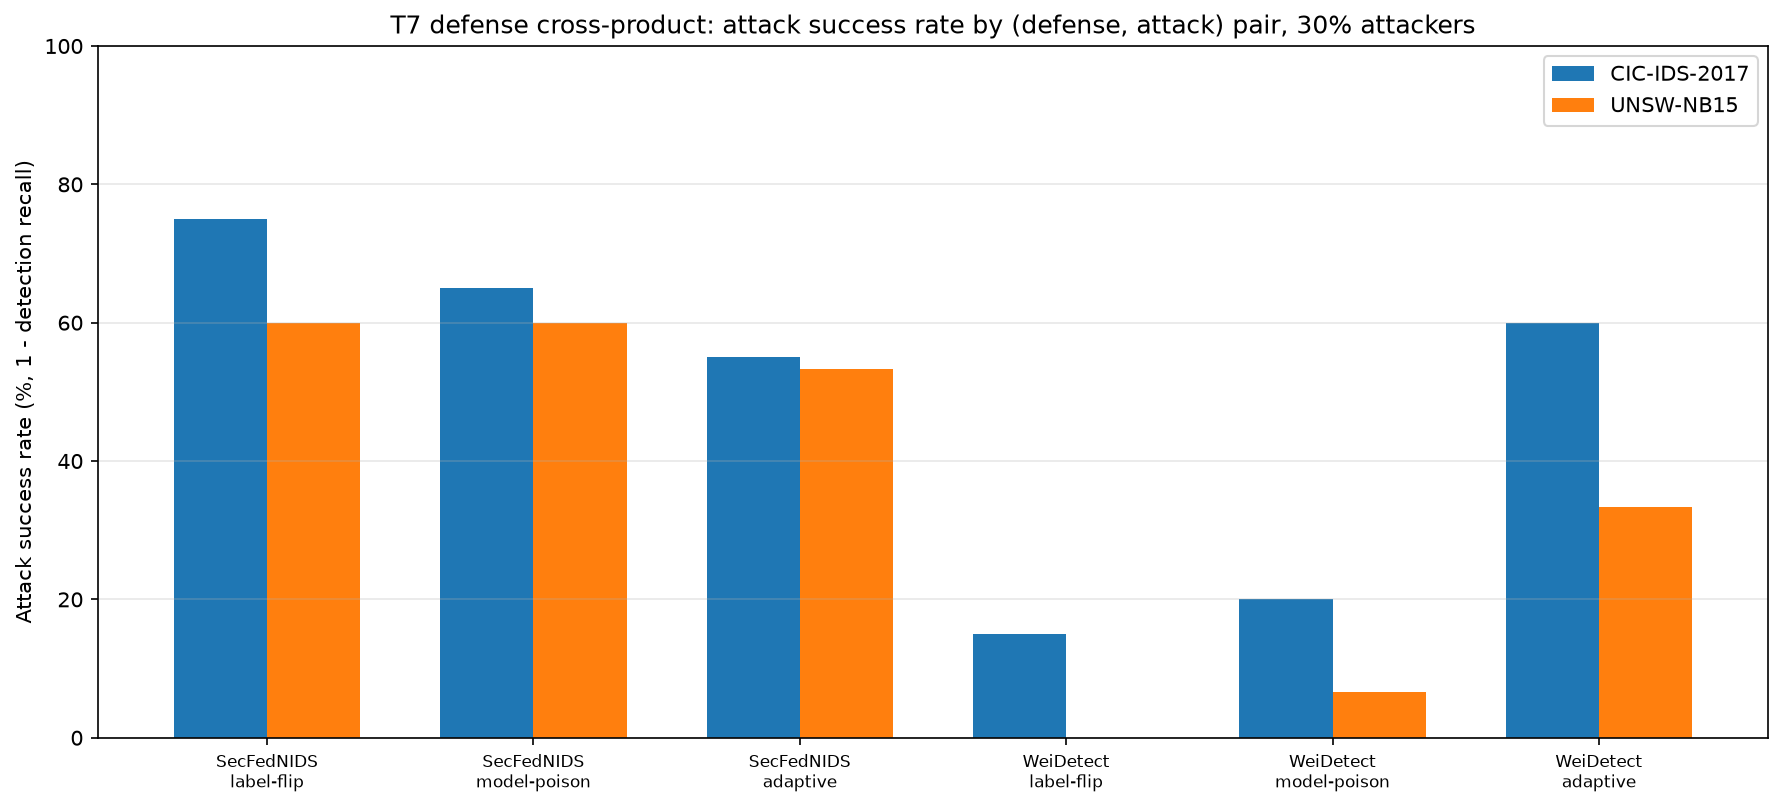
\includegraphics[width=0.74\textwidth]{figures/t7_defense_asr.png}
  \caption{Attack success rate for the two external defenses across the three
  attack types (lower is better for the defense).}
  \label{fig:t7-asr}
\end{figure}

The most consequential robustness finding, however, is not the detection
rates but the collateral damage. In every cell where a defense successfully
detects and excludes the attackers, the defense falls back to unweighted
averaging over the retained clients - which discards FedGRAA-v2's
rare-class-sensitive weighting along with the poison. The cost is exact and
measurable: across the 60 defended cells (2 defenses $\times$ 3 attacks
$\times$ 2 datasets $\times$ 5 seeds), rare-class recall is exactly 0.0\% in
\textbf{30 of 30 CIC cells} and \textbf{19 of 30 UNSW cells} (the remaining
11 UNSW cells retain partial recall, up to 33.3\%). Identical
\texttt{final\_all\_acc} values recur across different defended arms at the
same seed - e.g.\ all three UNSW label-flip defenses at seed~2 end at
exactly 0.49682 - mechanistic confirmation that each defense collapses to
the same unweighted fallback. The defended model is, on the metric the
entire system exists to serve, no better than FedAvg. AdaAggRL, the
reinforcement-learning baseline that learns protective weights, exhibits
the same failure under 30\% label-flipping: exactly 0.0\% rare-class recall
on all five CIC seeds and a 2.00\% mean on UNSW (one nonzero seed at
10.0\%). A defense that stops poisoning by discarding the mechanism's own
signal is not, in this evaluation, a free win - closing that gap is future
work, not a solved problem.

% =====================================================================
%  CHAPTER 5 -- DISCUSSION
% =====================================================================
\chapter{Discussion}
\label{ch:discussion}

\section{What the reproduction actually showed}
\label{sec:what-showed}

The internship's central finding is a three-layer result. The original
FedGRAA mechanism is directionally sound - adaptive, loss-driven
re-weighting on a simplex is a reasonable answer to rare-class starvation
under extreme non-IID partitioning - but the printed algorithm omits the
one step that keeps its own correctness argument valid. Restoring that step
(Euclidean projection, plus a feasible learning rate) recovers and exceeds
the paper's claimed performance, and replacing the two privacy assumptions
it inherited (oracle knowledge of the rare classes; a server-held labelled
validation set) costs nothing in accuracy while introducing a bounded,
decomposable gradient error $\zeta$ that the corrected convergence
proposition absorbs explicitly.

Equally important is what the reproduction did \emph{not} show. The literal
algorithm does not reproduce the printed headline numbers on any cell - it
collapses below the CIC claim while overshooting UNSW's, seed-unstably; the
paper's repeating-decimal table values (88.88, 77.77, 66.66,
33.33 - the 8/9, 7/9, 2/3, 1/3 fractions) are unverifiable and
pattern-inconsistent with measurements; and the
published theorem claims a global-optimality guarantee that the corrected
analysis does not restore - what is provable is stationarity of the
projected gradient mapping, a strictly weaker and honest statement.

\section{Reading the mechanism: three consequences}
\label{sec:reading-mechanism}

Three consequences emerge only when the Stage C results are read together
rather than as independent tables.

\paragraph{The $\gamma$ trade-off and the attack surface are the same
mechanism.} FedGRAA deliberately up-weights the clients whose updates most
reduce the rare-class-sensitive composite loss; Section~\ref{sec:adversarial}
shows an adversary exploits exactly that scoring rule, because a fabricated
rare-class signature is, to the weight learner, indistinguishable from a
genuine one. The protection and the exposure are not two properties of the
method - they are one. The T7G sweep sharpens this: the effect is
non-monotonic in $\gamma$, peaking near $\gamma = 0.5$ where the objective
genuinely mixes protected and unprotected strata rather than at the fully
rare-focused $\gamma = 1$, and collapsing to a coin-flip at $\gamma = 0$
where the protected term vanishes. That is consistent with a threshold
reading - the rare-class signal the attack rides on is reliably present only
above some $\gamma$ - but the 3-point, 2-fraction, 2-dataset grid is not
powered to confirm it, so it is stated as a hypothesis, not a result.

\paragraph{No evaluated defense is free.} The two external defenses stop the
attack only by discarding the signal FedGRAA-v2 exists to amplify: once
SecFedNIDS or WeiDetect filters a client set it falls back to
\emph{unweighted} averaging of the survivors, abandoning rare-class-sensitive
re-weighting entirely. The cost is measured, not asserted - 30/30 CIC and
19/30 UNSW defended cells collapse to exactly 0.0\% rare-class recall. A
defense that wins by removing the mechanism under evaluation is not a free
win; neither paper reports the trade-off because neither targets a
rare-class-sensitive aggregator. A filter that preserves the up-weighting
is, to our knowledge, open.

\paragraph{Exactness has a non-obvious price point.} The interesting answer
to ``is exactness worth it'' is not the $6.00\times$ headline at $m = 1$ but
$m = 3$: the cost halves to $3.00\times$ while rare-class recall
\emph{improves} (93.47\% vs.\ 88.06\% CIC; 69.66\% vs.\ 65.48\% UNSW), the
$\zeta_{\mathrm{stale}}(m)$ staleness acting as an implicit regularizer
rather than degrading. Against the data-free approximations - CELM and
SpectralFed cost a fraction of the traffic but return near-0\% rare recall
on CIC - exactness buys a capability the cheap methods lack, and at $m = 3$
it buys it at half the worst-case price.

\section{Engineering lessons}
\label{sec:lessons}

Several process findings generalize beyond this project.

\paragraph{No silent patching.} The repository keeps the literal
\texttt{FedGRAA} class unprojected on purpose, and implements the fix as a
separate \texttt{ProjectedFedGRAA}. This strict-reproduction boundary is
what makes the Stage A versus Stage B comparison an experiment rather than
an assertion: the failure and the fix are both measured, and neither is
contaminated by the other.

\paragraph{Audit scripts, not summaries.} Each stage carries an independent
\texttt{audit\_stage\_*.py} that re-derives every reported number from raw
JSON rather than trusting the documents - and the audits found real defects
(six summarization defects in Stage~B alone, a HIGH-severity transcription
error in the Stage~C manuscript prose at 50\% attacker fraction, zero
numerical errors in computed results). Every number in this report was
either read from a generated table or recomputed from raw JSON the same
way.

\paragraph{Negative results are the evidence.} The 111/112 significance
count, the 19/30 partial UNSW collapse, the bimodal $\gamma = 0$ attack
surface, and the literal arm's 0.4-44.0\% seed spread are all reported at
full precision because each is a finding in its own right. Rounding
111/112 to ``all significant'' or the UNSW collapse to ``all cells'' would
have been wrong in exactly the way the original paper was wrong.

\paragraph{Discrepancy handling is part of the deliverable.} The project
documents, rather than hides, its source disagreements: the UNSW input
width (43 printed versus 39 implemented), the two different formulas both
called ``FedAvg'' in the original manuscript, the SGD-versus-Adam
client-update contradiction, the retracted PDF-to-Markdown hallucination
finding, and the test-count snapshots that differ across stage boundaries.
Where the counts differ, each number is attributed to its snapshot rather
than silently reconciled.

\section{Limitations and honest caveats}
\label{sec:limitations}

\begin{itemize}
  \item \textbf{Threat model.} FedGRAA-v2 assumes an honest-but-curious
  server, the standard SecAgg collusion threshold, and $f < K/3$ dropout
  tolerance. A fully malicious server, Byzantine clients, and verifiable
  SecAgg are explicitly out of scope.
  \item \textbf{Plaintext parameter channel.} The training updates
  $\theta_k^t$ remain plaintext; DLG-style gradient inversion
  \cite{zhu2019dlg} applies to them regardless of the SecAgg-protected
  channels. This is a pre-existing surface, not one the redesign closed.
  \item \textbf{Small-$K$ SecAgg thresholds.} At $K = 9$-14 the default
  reconstruction threshold is a bare majority $t = \lfloor K/2 \rfloor + 1$
  ($t = 8$ on the 14-client CIC split, $t = 5$ on the 9-client UNSW split),
  tolerating 6 and 4 dropouts respectively; a stricter
  $t = \lceil 2K/3 \rceil$ deployment choice would tolerate only 3-4. Either
  way, a server colluding with $K{-}1$ clients recovers the last
  contribution by subtraction, so the privacy guarantee is thinner at this
  scale than at Google-scale deployments.
  \item \textbf{PL is a stated condition, not a verified one.} The
  $\zeta$-inexact theorem conditions its rate on the Polyak-Lojasiewicz
  property holding on $\Delta$ for this loss surface; the manuscript states
  this as the correct condition to check, and does not claim to have
  verified it. Three rigor flags remain for a referee-grade pass:
  $\beta_{\mathrm{eff}}$ is unestimated, the $\min(\cdot,\cdot)$
  subdifferential is handled by sketch, and the $O(1/T)$ constant is not
  explicit.
  \item \textbf{Staleness is bounded, not eliminated.} The federated
  gradient is exact \emph{at each refresh}; at $m > 1$ the between-refresh
  staleness term $\zeta_{\mathrm{stale}}(m)$ is absorbed by the theorem,
  not removed.
  \item \textbf{Statistical floor.} Ten seeds cap the attainable Wilcoxon
  $p$-value at $0.001953$; several ``significant'' findings sit exactly at
  that floor and would benefit from more seeds.
  \item \textbf{SecFedNIDS is a weak reproduction.} Its 53-75\% ASR on
  these datasets is far from its published UNSW-NB15/CSE-CIC-IDS2018
  detection rates; whether that reflects the datasets, the attack grid, or
  the implementation is unresolved.
  \item \textbf{Provenance unresolved.} Whether the original manuscript was
  ever formally published remains open (DBLP returns zero hits); this does
  not affect the algorithmic findings but blocks treating it as a peer
  artifact.
  \item \textbf{Known deviation.} Client-side Adam momentum persists across
  all 200 rounds while client parameters reset each round - documented as
  a deviation, orthogonal to the projection fix, and not corrected by it.
  \item \textbf{$\gamma$ is manual, not learned.} The common-versus-rare
  trade-off is set by a hand-chosen $\gamma$; Section~\ref{sec:adversarial}
  shows the attack surface itself is $\gamma$-sensitive (peaking near
  $\gamma = 0.5$, bimodal at $\gamma = 0$), so no single fixed value is
  uniformly best across objectives. Automating that trade-off is future
  work, not done here.
  \item \textbf{Small scale.} All results use $n = 3$ protected classes and
  $K = 9$-14 clients on synthetic non-IID partitions of two public datasets;
  a real cross-silo deployment (50-200 silos, genuinely heterogeneous
  organizations, on a corpus such as NF-UQ-NIDS-v2) is untested and the
  per-client-one-attack partition is an extreme, not representative, case.
  \item \textbf{Classic-optimizer theory gap.} The SCAFFOLD and FedNova
  baselines are run with the same Adam local solver as everything else for
  comparability, while their published convergence guarantees assume an SGD
  local update; their measured numbers are therefore honest empirical
  results, not tests of their own theorems.
  \item \textbf{Ideal-functionality SecAgg.} The module models the
  Bonawitz interface contract (sums only, threshold, dropout error), not
  the cryptographic protocol itself.
\end{itemize}

\section{Future work}
\label{sec:future}

The natural continuations, in roughly increasing order of scope: (i)
referee-grade hardening of the corrected proposition - estimating
$\beta_{\mathrm{eff}}$, a formal Clarke-subdifferential treatment of the
$\min(\cdot,\cdot)$ arm selection, and an explicit $O(1/T)$ constant; (ii)
a defense that stops poisoning \emph{without} discarding the rare-class
signal - the filtering layer of Jiang et al.\ \cite{jiang2024} is the
closest precedent, and
the defended-cell collapse of Section~\ref{sec:adversarial} is precisely
the gap it would need to close; (iii) real cross-silo evaluation on
NF-UQ-NIDS-v2, for which the four-silo partitioner and the bounded-memory
loader already exist (T6 runs the T1 grid at 4 clients); (iv) verifiable
SecAgg to remove the honest-execution assumption; and (v) the project's
documented Option A - a few-shot/prototype-guided hybrid combining
FedGRAA's gradient refinement with prototype exchange - which the
remaining-compute plan identifies as a second, independent novelty
contribution but which is deliberately not started pending a design/theory
document.

% =====================================================================
%  CHAPTER 6 -- CONCLUSION
% =====================================================================
\chapter{Conclusion}
\label{ch:conclusion}

{\sloppy
This internship set out to reproduce, diagnose, correct, and extend a
federated-learning intrusion-detection paper, and to evaluate the result
under the statistical and adversarial scrutiny the original publication
did not receive. Each of the five objectives closed with a measured
answer.\par}

\textbf{O1 - Faithful reproduction.} The printed FedGRAA algorithm was
implemented literally, with every documented ambiguity resolved by the
code-level reading rather than patched over. The literal implementation
reproduces none of the paper's headline numbers: 0.00\% versus a claimed
88.88\% rare-class accuracy on CIC-IDS-2017 at $\gamma = 1$, and 33.33\%
versus a claimed 21.09\% on UNSW-NB15 - the latter an inversion in which
the reproduction beats the claim while its loss diverges.

\textbf{O2 - Diagnosis.} The failure is a missing Euclidean projection
onto the probability simplex. The printed update is an unconstrained
descent over $\mathbb{R}^K$ while the paper's own lemma assumes
$w \in \Delta$; the iterate leaves the simplex at round~1 in 120 of 120
unprojected cells, and the composite loss diverges by up to six orders of
magnitude. The printed proof fails on three compounding grounds: convexity
assumed for a non-convex tanh-MLP, no finite smoothness constant at the
$\min(\cdot,\cdot)$ kink, and a tacit feasibility assumption nothing
enforces.

\textbf{O3 - Corrected theory.} Projected subgradient descent
$w^t = \Pi_\Delta(w^{t-1} - \eta' \partial L'(w^{t-1}))$ with
$\eta' = 0.01$ restores feasibility structurally - 0 of 120 projected cells
violate - and the corrected guarantee is gradient-mapping stationarity,
$\min_{t \leq T} \|G_{\eta'}(w^t)\|^2 = O(1/T)$, stated honestly as weaker
than the paper's global-optimality claim. The Stage B factorial showed the
fix is the only arm never catastrophically wrong on either metric, on
either dataset, at any $\gamma$.

\textbf{O4 - Privacy-compliant extension.} FedGRAA-v2 removes the
manuscript's two privacy assumptions - oracle rare-class knowledge and a
server-held labelled validation set - via SecAgg-summed label histograms
and a two-phase federated backward pass that is algebraically identical
to the pooled computation ($\tilde{\zeta} \lesssim 4\times10^{-7}$). The
$\zeta$-inexact proposition generalizes the convergence result to
$O(1/T) + O(\zeta^2)$.

\textbf{O5 - Statistically tested evaluation.} Across the 960-cell Stage C
campaign, the best v2 arm ($m = 3$) reaches 93.47\% rare-class recall on
CIC-IDS-2017 and 69.66\% on UNSW-NB15 - exceeding the privacy-violating
oracle on both - at 3.00$\times$ FedAvg's communication cost, with 111 of
112 Holm-corrected comparisons significant. The adversarial campaigns
quantify the mechanism's own attack surface (up to $3.3\times$ uniform
attacker weight) and document, at full precision, the finding that in every
cell where an evaluated poisoning defense succeeds in stopping the attack,
it does so only by destroying the rare-class signal the system exists to
protect - 30/30 CIC defended cells and 19/30 UNSW defended cells collapse
to exactly 0.0\% rare recall.

The arc is therefore complete: the original mechanism works, once it is
made to do what its own proof assumed it did. The honest version of the
claim - a different, defensible point in an occupied design space, with an
evaluation axis no adjacent work reports - is the one this report stands
behind.

% =====================================================================
%  BIBLIOGRAPHY
% =====================================================================
\clearpage
\phantomsection\addcontentsline{toc}{chapter}{Bibliography}
\bibliographystyle{plain}
{\footnotesize
\setlength{\itemsep}{0pt}
\setlength{\parsep}{0pt}
\begin{spacing}{0.9}
\bibliography{references}
\end{spacing}
}

% =====================================================================
%  APPENDIX A -- REPRODUCIBILITY MANIFEST
% =====================================================================
\appendix
\chapter{Reproducibility Manifest}
\label{app:manifest}

This appendix records the artifact-level details needed to reproduce or
audit every number in this report. The project repository is
\texttt{github.com/N1KH1LT0X1N/FedGRAA} (MIT license); the working tree is
pinned at Python 3.13.14 with TensorFlow 2.21.0, Keras 3.15.0, NumPy 2.5.1,
SciPy 1.18.0, scikit-learn 1.9.0 and pytest 9.1.1.

\section{Artifact map}
\label{sec:artifact-map}

Every quantitative claim in this report traces to one of the generated
artifacts or raw result files in Table~\ref{tab:provenance}:

\begin{table}[htbp]
  \centering
  \caption{Figure and table provenance.}
  \label{tab:provenance}
  \footnotesize
  \begin{tabular}{@{}ll@{}}
    \toprule
    Report item & Source artifact(s) \\
    \midrule
    Figs.~\ref{fig:cic-gamma-sweep}, \ref{fig:unsw-gamma-sweep}, \ref{fig:cic-nsweep}, \ref{fig:unsw-nsweep}
      & \texttt{results/\{DS\}\_gamma\_sweep.json}, \texttt{\{DS\}\_n\_sweep.json} \\
    Fig.~\ref{fig:diagnosis}
      & \texttt{results/diagnosis/}, \texttt{fedgraa\_convergence\_defect.md} \S2 \\
    Figs.~\ref{fig:ablation-cic}, \ref{fig:ablation-unsw};
    Tabs.~\ref{tab:ablation}, \ref{tab:factorial}
      & \texttt{results/ablation/*\_ablation\_table.md} + raw JSON \\
    Fig.~\ref{fig:frontier}; Tab.~\ref{tab:frontier}
      & \texttt{results/v2\_frontier/frontier\_table.md} + raw JSON \\
    Fig.~\ref{fig:classic-fl} & \texttt{results/v2\_frontier/} (classic arms) \\
    Fig.~\ref{fig:overhead}; Tab.~\ref{tab:overhead}
      & \texttt{results/v2\_frontier/overhead\_table.md} \\
    \S\ref{sec:significance} & \texttt{results/v2\_frontier/significance\_table.md} (112 rows) \\
    Fig.~\ref{fig:t7-weights}; Tab.~\ref{tab:t7g}
      & \texttt{results/v2\_frontier/*raresig*.json}, \texttt{attacker\_weight\_history} \\
    Fig.~\ref{fig:t7-asr}; Tab.~\ref{tab:asr}
      & \texttt{results/v2\_frontier/\{secfednids,weidetect\}*.json} \\
    Defended-cell counts (\S\ref{sec:adversarial})
      & \texttt{final\_last\_n\_acc} of the 60 defended JSON cells \\
    \bottomrule
  \end{tabular}
\end{table}

\section{Campaign accounting}
\label{sec:campaign-accounting}

The Stage C campaign comprises 960 result cells, each persisted as a
self-describing JSON under \texttt{results/}: an 830-cell main grid (480
frontier/classic cells $=$ 24 arms $\times$ 2 datasets $\times$ 10 seeds,
plus 200 T2, 100 T4 and 50 T6 extension cells), a 90-cell T7 adversarial
grid and a 40-cell T7G attacker-side $\gamma$ sweep. Stage B comprises 240
diagnostic cells (4 arms $\times$ 2 datasets $\times$ 3 $\gamma$ $\times$ 10
seeds) plus 40 baseline seed-runs; Stage A comprises the 200-round seed-0
$\gamma$ and $n$ sweeps.

\section{Test suite}
\label{sec:test-suite}

The repository's verification gates, wired in
\texttt{.github/workflows/docs-check.yml}, are:
\begin{itemize}[nosep]
  \item \texttt{compileall} over \texttt{fedgraa}, \texttt{scripts} and
  \texttt{tests}; \texttt{pytest tests}; \texttt{check\_doc\_links.py};
  \item \texttt{check\_stage\_a\_complete.py} and
  \texttt{audit\_stage\_a.py} (Stage A);
  \item \texttt{check\_stage\_b\_complete.py} and
  \texttt{audit\_stage\_b.py} (Stage B);
  \item \texttt{check\_stage\_c\_complete.py} and
  \texttt{audit\_stage\_c.py} (Stage C; tiers \texttt{T1}-\texttt{T6} plus
  \texttt{TC} with \texttt{-{}-t4-m 3}, and \texttt{T7} at seeds 0-4).
\end{itemize}

Test-count references across documents are snapshots, not a single
invariant: 79 at the Stage A close, 142 at the Stage B close, 558 by
\texttt{-{}-collect-only} in the Stage C report's own recomputation, 563 in
that report's measured suite, and \textbf{565} collected on the current
working tree when the optional \texttt{matplotlib} and \texttt{modal}
dependencies are present (their absence cleanly skips 35
collection-time-gated tests: 7 plot, 6 render-ablation, 22 modal). One
script outside \texttt{tests/} is not part of the suite: the archived GPU
probe \texttt{scripts/archive/gpu/test\_gpu.py}, which fails on CPU-only
TensorFlow builds by design (its CUDA build-info key is absent).

\section{Re-derivation}
\label{sec:rederive}

Each stage ships an independent audit that recomputes its reported numbers
from raw JSON rather than trusting the documents: \texttt{audit\_stage\_a},
\texttt{audit\_stage\_b} (SHA-256 manifest check, per-seed exact compare,
SciPy recomputation of the 60 pairwise comparisons and 18 factorial
effects, and 262 doc-transcribed numbers) and \texttt{audit\_stage\_c}.
The exactness of
the two-phase gradient protocol is enforced by
\texttt{tests/test\_aggregation\_v2.py} (relative error $< 10^{-6}$) and
measurable end-to-end via \texttt{scripts/verify\_v2\_exactness.py}; the
byte-formula of Eq.~\eqref{eq:overhead} is enforced by
\texttt{test\_measured\_bytes\_match\_frontier\_formula}.

\end{document}
